\documentclass[conference]{IEEEtran}
\IEEEoverridecommandlockouts
% The preceding line is only needed to identify funding in the first footnote. If that is unneeded, please comment it out.
\usepackage{cite}
\usepackage{amsmath,amssymb,amsfonts}
\usepackage{algorithmic}
\usepackage{graphicx}
\usepackage{subcaption}
\usepackage{textcomp}
\usepackage{xcolor}
\usepackage[utf8]{inputenc}
\usepackage[vietnamese]{babel}
\usepackage{amsmath}
\usepackage{float}
\usepackage{natbib}
\usepackage{multirow}
\usepackage{multicol}
\usepackage{makecell}
\usepackage{booktabs}
\usepackage{array}
\usepackage{hyperref}
\setlength{\parskip}{0pt}
\setlength{\parindent}{0pt}
\setlength{\baselineskip}{0em}
\setlength{\abovedisplayskip}{0pt}
\setlength{\belowdisplayskip}{0pt}

\def\BibTeX{{\rm B\kern-.05em{\sc i\kern-.025em b}\kern-.08em
    T\kern-.1667em\lower.7ex\hbox{E}\kern-.125emX}}
\usepackage[backend=bibtex,style=ieee]{biblatex}
\addbibresource{ref.bib}

\begin{document}

\title{Dự báo giá cổ phiếu ngân hàng Việt Nam bằng các mô hình Thống kê, Máy học và Học sâu\\}
\author{
    \IEEEauthorblockN{
        \begin{minipage}{\textwidth}
            \centering
            \begin{minipage}{0.3\textwidth}
                \centering
                1\textsuperscript{st} Trần Ngọc Tố Như\\
                \textit{Khoa Hệ thống thông tin,}\\
                \textit{Trường Đại học Công nghệ thông tin-ĐHQG}\\
                21520385@gm.uit.edu.vn
            \end{minipage}
            \hfill
            \begin{minipage}{0.3\textwidth}
                \centering
                2\textsuperscript{nd} Lê Thùy Dương\\
                \textit{Khoa Hệ thống thông tin,}\\
                \textit{Trường Đại học Công nghệ thông tin-ĐHQG}\\
                21520203@gm.uit.edu.vn
            \end{minipage}
            \hfill
            \begin{minipage}{0.3\textwidth}
                \centering
                3\textsuperscript{rd} Trần Thanh Huy\\
                \textit{Khoa Hệ thống thông tin,}\\
                \textit{Trường Đại học Công nghệ thông tin-ĐHQG}\\
                21522170@gm.uit.edu.vn
            \end{minipage}
        \end{minipage}
        \\[1.5em] % khoảng cách giữa hai hàng
        \begin{minipage}{\textwidth}
            \centering
            \begin{minipage}{0.45\textwidth}
                \centering
                4\textsuperscript{th} Mai Trần Khương Duy\\
                \textit{Khoa Hệ thống thông tin,}\\
                \textit{Trường Đại học Công nghệ thông tin-ĐHQG}\\
                21521998@gm.uit.edu.vn
            \end{minipage}
            \hfill
            \begin{minipage}{0.45\textwidth}
                \centering
                5\textsuperscript{th} Vũ Tiến Linh\\
                \textit{Khoa Hệ thống thông tin,}\\
                \textit{Trường Đại học Công nghệ thông tin-ĐHQG}\\
                19521760@gm.uit.edu.vn
            \end{minipage}
        \end{minipage}
    }
}
\maketitle

\begin{abstract}
Việc tích hợp công nghệ thông tin vào các khía cạnh khác nhau của cuộc sống, bao gồm kinh tế, y tế và thương mại, ngày càng trở nên phổ biến. Nhất là trong các lĩnh vực được quan tâm đặc biệt, nhu cầu ứng dụng mạnh mẽ công nghệ thông tin ngày càng tăng cao, đặt ra thách thức cho những người làm trong ngành công nghệ thông tin. Một trong những bài toán được quan tâm hiện nay là việc dự đoán giá cổ phiếu của các tổ chức ngân hàng. Báo cáo này tập trung vào dự đoán giá cổ phiếu của ba ngân hàng: BIDV, VCB và MBB, sử dụng nhiều thuật toán thuộc nhiều loại khác nhau, bao gồm các thuật toán học sâu, thuật toán máy học và thuật toán thống kê (Linear Regression, Holt-Winter, ARIMA, XGBoost, Linear Regression với CalendarFourier, DeterministicProcess, MICN, CNN-LSTM, RNN, GRU, LSTM) để dự đoán, đồng thời so sánh, đánh giá kết quả khi sử dụng những thuật toán nêu trên.
\end{abstract}

\begin{IEEEkeywords}
Stock, Linear Regression, Holt-Winter, ARIMA, XGBoost, Linear Regression Calendar Fourier, Deterministic, RNN, GRU, LSTM, CNN-LSTM, MICN
\end{IEEEkeywords}

\section{GIỚI THIỆU}
Trong bất kỳ quốc gia nào, thị trường trứng khoán đóng vai trò quan trọng trong nền kinh tế của mỗi quốc gia, thị trường chứng khoán Việt Nam xem là tương đối trẻ so với các quốc gia trên toàn cầu. Sự bùng nổ về trí tuệ nhân tạo và học máy đã thúc đẩy sự quan tâm của các nhà đầu tư cá nhân, tổ chức vào việc tận dụng các công nghệ này để dự đoán thị trường chứng khoán nói chung và giá cổ phiếu nói riêng tại Việt Nam. 

Do đó trong nghiên cứu này, nhóm sẽ đi sâu vào việc áp dụng các thuật toán thống kê, máy học, học sâu khác nhau như Linear Regression, Holt-Winters, ARIMA, Recurrent Neural Network (RNN), Gated Recurrent Unit (GRU), Long Short-Term Memory (LSTM), Extreme Gradient Boosting (XGBoost), Linear Regression áp dụng CalendarFourier, DeterministicProcess, Convolutional Neural Network - Long Short-Term Memory (CNN-LSTM) và Multi-Channel Neural Networks (MICN), đồng thời cũng đánh giá hiệu suất của các thuật toán nêu trên. 

Trong nghiên cứu này, nhóm chọn ngành ngân hàng là vì nó có tác động trực tiếp đến nền kinh tế của đất nước. Ngoài ra, cổ phiếu ngân hàng còn đại diện cho một ngành ổn định với vốn hóa thị trường đáng kể trên sàn giao dịch chứng khoán Việt Nam. Nghiên cứu tập trung vào dự đoán giá cổ phiếu cho ba ngân hàng lớn được niêm yết trên thị trường chứng khoán Việt Nam hiện nay là BIDV, VCB và MBB.

\section{CÁC CÔNG TRÌNH NGHIÊN CỨU LIÊN QUAN}
Trong những năm qua, việc xác định dữ liệu chứng khoán rất phức tạp, do đó có rất nhiều phương pháp dự đoán chuỗi thời gian đã được đề xuất. Điển hình, theo \cite{predictStockCNNLSTM} nhóm tác giả đã sử dụng CNN-LSTM để đưa ra dự đoán cổ phiếu của một công ty trên thị trường chứng khoán nếu biết được những thông tin trước đó. Độ chính xác của mô hình CNN-LSTM được đánh giá là cao ngay cả khi huấn luyện trên dữ liệu thị trường chứng khoán theo thời gian thực. Bằng cách chuyển đổi dữ liệu chứng khoán thành dạng tensor (dữ liệu nhiều hơn 2 chiều) và sau đó gửi nó tới mạng thần kinh LSTM để tìm ra các mẫu. Từ đó dự đoán cổ phiếu thị trường trong một khoảng thời gian nhất định.

Mặt khác, Poongodi M, Vijayakumar V và Naveen Chilamkurti đã thu thập dữ liệu về bitcoin blockchain từ ngày 28/04/2013 đến ngày 31/07/2017 có sẵn công khai trên
\href{https://coinmarketcap.com}{https://coinmarketcap.com} và áp dụng mô hình ARIMA để dự đoán giá bitcoin \cite{predictBitcoinARIMA}.

Các nghiên cứu trước đây đã khám phá các phương pháp khác nhau để giải quyết nhiệm vụ khó khăn của việc dự đoán giá cổ phiếu. \cite{randomForestAndLSTM} Nghiên cứu đã đề xuất một mô hình kết hợp bằng cách sử dụng mạng nơ-ron hồi quy (RNN) với Random Forest, thể hiện sự cải thiện đáng kể trong dự báo giá cổ phiếu.

Trong một bài báo khác, Xiwen Jin và Chaoran Yi đã kết luận rằng LSTM và GRU cho kết quả tương đối tốt hơn và Random Forest là tệ nhất. Điểm R2 cho các mô hình khác nhau mà các tác giả đã phân tích: LSTM 0.84, GRU 0.86, mô hình Hồi quy Random Forest 0.51, mô hình Hồi quy XGBoost 0.69, Hồi quy Tuyến tính 0.73 và mô hình Hồi quy LGBM 0.72. Từ đó có thể thấy rằng XGBoost và Random Forest có hiệu suất không tốt bằng  các mô hình LSTM và GRU \cite{comparationLinearRegression}.

MICN mang lại sự cải thiện 17,2\% và 21,6\% cho phương pháp đa biến. Sử dụng kết hợp CNN và Transformers để hướng tới mục tiêu sử dụng thông tin tổng thể của đầu vào một cách hiệu quả. Trước tiên là trích xuất đặc trưng cục bộ của dữ liệu, sau đó lập mô hình mối tương quan toàn cầu trên cơ sở này \cite{MICN}.

Awajan, Ismail và Alwadi đã phát triển phương pháp EMD-HW bằng cách kết hợp Empirical Mode Decomposition và Holt-Winter để dự đoán thị trường chứng khoán. Dữ liệu chứng khoán được phân rã thành các Intrinsic Mode Functions (IMFs) và các phần dư còn lại. Tất cả các thành phần được dự báo bằng kỹ thuật Holt - Winter. Các giá trị dự báo sẽ được tổng hợp để có giá trị dự đoán cho thị trường chứng khoán. Điểm mạnh của EMD-HW này nằm ở khả năng dự đoán các chuỗi thời gian không ổn định và phi tuyến mà không cần sử dụng bất kỳ phương pháp biến đổi nào \cite{forecastingHoltWinter}.
\section{TẬP DỮ LIỆU}}
\subsection{MÔ TẢ TỔNG QUAN}}
Lịch sử giá cổ phiếu của 3 ngân hàng: Ngân hàng Thương mại cổ phần Đầu tư và Phát triển Việt Nam (BIDV), ngân hàng thương mại cổ phần Ngoại thương Việt Nam (VCB), ngân hàng Thương mại cổ phần Quân đội (MBB). Dữ liệu được lấy từ ngày 1 tháng 1 năm 2018 đến ngày 1 tháng 6 năm 2024. Mỗi bộ dữ liệu chứa khoảng 1555 dòng và bao gồm 7 thuộc tính: Date, Price, Open, High, Low, Vol, Change.
Trong đó: 
\begin{itemize}
    \item Date: Ngày giao dịch 
    \item Price: Giá trị cuối cùng của cổ phiếu tại giờ đóng cửa
    \item Open: Giá mở cửa của cổ phiếu tại ngày giao dịch
    \item High: Giá cao trị cao nhất mà cổ phiếu đạt đến trong ngày 
    \item Low: Giá thấp nhất mà cổ phiếu đạt được trong ngày
    \item Vol: Khối lượng giao dịch của cổ phiếu trong ngày (đơn vị: triệu cổ phiếu)
    \item Change: Sự chênh lệch của giá đóng cửa so với giá đóng cửa của ngày trước đó (giá trị %)
\end{itemize}


\subsection{THỐNG KÊ MÔ TẢ}
\begin{table}[htbp]
\caption{BIDV, VCB, MBB’s Descriptive Statistics}
\begin{center}
\begin{tabular}{|c|c|c|c|}
\hline
\textbf{} & \textbf{\textit{BIDV}} & \textbf{\textit{VCB}} & \textbf{\textit{MBB}} \\
\hline
Count & 1598 & 1598 & 1598 \\
\hline
Mean & 33466.789 & 67714.813 & 15575.501 \\
\hline
Std & 7261.683 & 14916.299 & 5360.553 \\
\hline
Min & 16531.4 & 35483 & 7206.6 \\
\hline
25\% & 28166.65 & 55687.75 & 10936.525 \\
\hline
50\% & 32375.3 & 67731 & 14605.7 \\
\hline
75\% & 38500 & 78577 & 18786.2 \\
\hline
Max & 54400 & 97400 & 28666.7 \\
\hline
\end{tabular}
\label{tab1}
\end{center}
\end{table}

\begin{minipage}{0.21\textwidth}
    \centering
    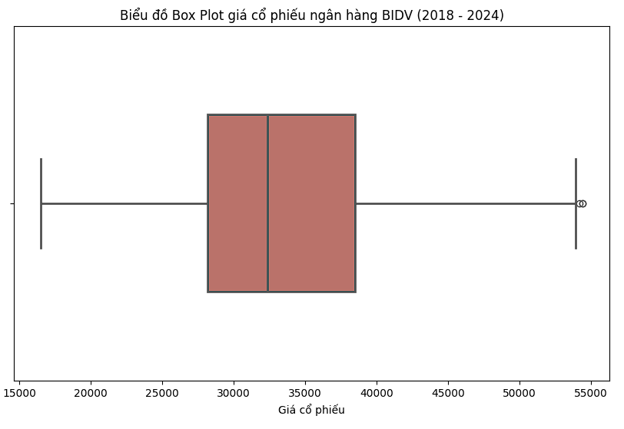
\includegraphics[width=\linewidth]{images/Statistic/bidv_boxplot.png}
    \captionof{figure}{Box Plot of BIDV stock price (2018 - 2024)}
    \label{fig:image1}
\end{minipage}
\hfill
\begin{minipage}{0.21\textwidth}
    \centering
    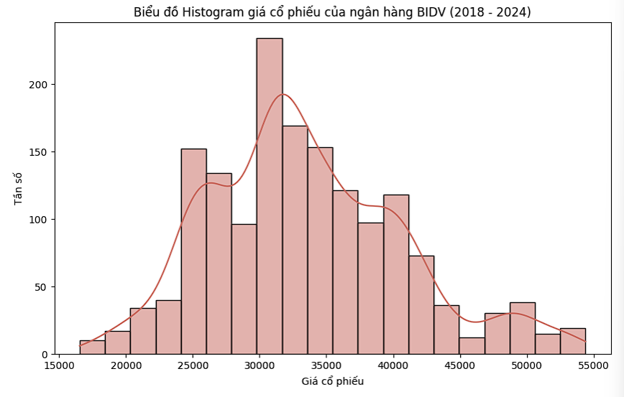
\includegraphics[width=\linewidth]{images/Statistic/bidv_histogram.png}
    \captionof{figure}{Histogram of BIDV Stock Price (2018 - 2024)}
    \label{fig:image2}
\end{minipage}

\begin{minipage}{0.21\textwidth}
    \centering
    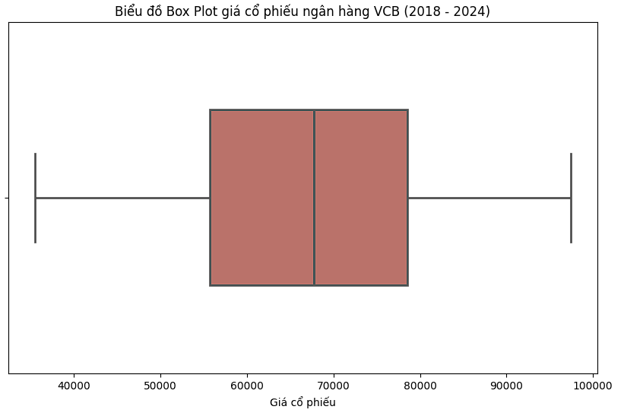
\includegraphics[width=\linewidth]{images/Statistic/vcb_boxplot.png}
    \captionof{figure}{Box Plot of VCB Stock Price (2018 - 2024)}
    \label{fig:image1}
\end{minipage}
\hfill
\begin{minipage}{0.21\textwidth}
    \centering
    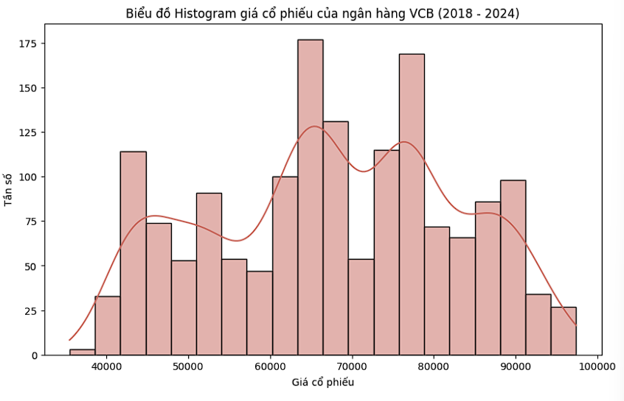
\includegraphics[width=\linewidth]{images/Statistic/vcb_histogram.png}
    \captionof{figure}{Histogram of VCB Stock Price (2018 - 2024)}
    \label{fig:image2}
\end{minipage}

\begin{minipage}{0.21\textwidth}
    \centering
    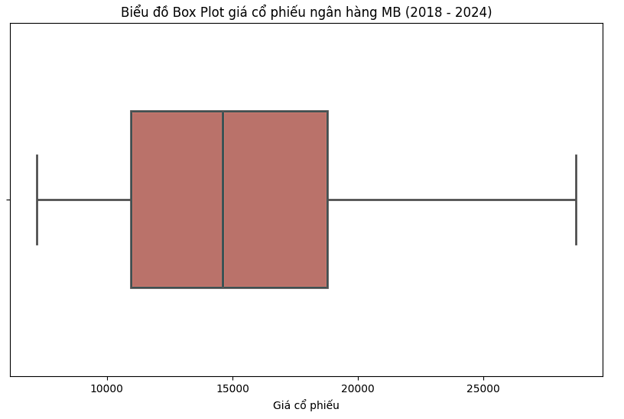
\includegraphics[width=\linewidth]{images/Statistic/mbb_boxplot.png}
    \captionof{figure}{Box Plot of MB Bank Stock Price (2018 - 2024)}
    \label{fig:image1}
\end{minipage}
\hfill
\begin{minipage}{0.21\textwidth}
    \centering
    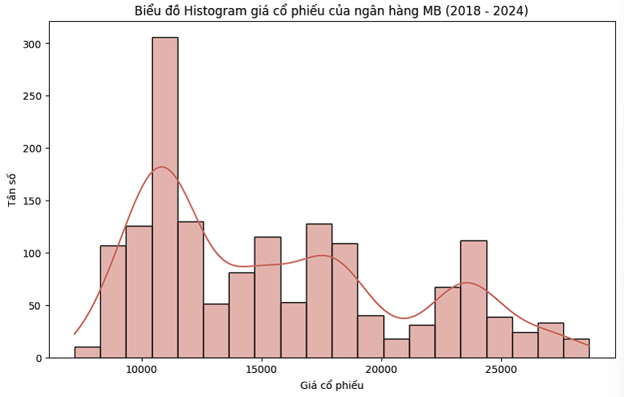
\includegraphics[width=\linewidth]{images/Statistic/mbb_histogram.png}
    \captionof{figure}{Histogram of MB Bank Stock Price (2018 - 2024)}
    \label{fig:image2}
\end{minipage}



\section{PHƯƠNG PHÁP LUẬN}
\subsection{ARIMA}
Mô hình ARIMA là là sự kết hợp của quá trình từ hồi quy (Auto Regression – AR), quá trình trung bình trượt (Moving Average - MA) và Tính hợp sai phân (Integrated – I). Mô hình ARIMA chỉ hoạt động tốt nếu dữ liệu phụ thuộc nhiều vào thời gian và trong chuỗi dữ liệu dừng. Những dữ liệu dạng ngẫu nhiên thường ít hoạt động tốt đối với mô hình ARIMA. Mô hình ARIMA cần bộ dữ liệu có tính dừng, nếu không có tính dừng, cần tích hợp sai phân để làm bộ dữ liệu có tính dừng.\\
Chuỗi dừng: Một chuỗi thời gian có tính dừng  là một chuỗi các giá trị Mean, Variance, Autocorrelation không thay đổi theo thời gian và nó không bao hàm yếu tố xu hướng.\\
Mô hình ARIMA không có tính mùa vụ: được biểu diễn với ký hiệu tiêu chuẩn được sử dụng là ARIMA(p,d,q)
\begin{itemize}
    \item I(d) Integrated so sánh sự khác nhau giữa d quan sát, hiệu giữa giá trị hiện tại và d giá trị trước đó. Quá trình sai phân được thực hiện: \\
    Sai phân bậc 1:\(I(1) = \Delta y_t = y_t - y_{t-1}\) \\
    Sai phân bậc 2:\(I(2) = \Delta^2 y_t = (y_t - y_{t-1}) - (y_{t-1} - y_{t-2})\) \\
    Sai phân bậc d được ký hiệu là I(d)
    \item AR(p) Autoregression: là quá trình tìm mối quan hệ giữa dữ liệu hiện tại và p dữ liệu quá khứ trước đó gọi là (Lag) được biểu diễn với công thức. 
    \[y_t = a_0 + a_1 y_{t-1} + a_2 y_{t-2} + \cdots + a_p y_{t-p} + \epsilon_t\]
    Điều kiện dừng của việc chọn \( p \): \(\sum_{i=0}^p a_i < 1\)
    \item MR(q) Moving Average là quá trình tìm mối quan hệ giữa dữ liệu hiện tại và q phần lỗi quá khứ trước đó được biểu diễn với công thức
    \[
    y_t = \beta_0 + \beta_1 \epsilon_{t-1} + \beta_2 \epsilon_{t-2} + \cdots + \beta_q \epsilon_{t-q} + \mu_t
    \]
    Điều kiện dừng của việc chọn \( q \):\(\sum_{i=0}^q \beta_i < 1\)
\end{itemize}
\subsection{Linear Regression}
Hồi quy tuyến tính là một phương pháp thống kê để mô hình hóa mối quan hệ giữa một biến phụ thuộc và một hoặc nhiều biến độc lập. Thuật toán tìm đường thẳng tốt nhất để dự đoán giá trị của biến phụ thuộc dựa trên các biến độc lập, sao cho sai số giữa kết quả dự đoán và giá trị thực tế của biến phụ thuộc là nhỏ nhất. Mô hình hồi quy tuyến tính có hai dạng chính: hồi quy tuyến tính đơn biến và hồi quy tuyến tính đa biến.\\
Hồi quy tuyến tính đơn biến chỉ sử dụng một biến độc lập, trong khi hồi quy tuyến tính đa biến sử dụng nhiều hơn một biến độc lập. Hồi quy tuyến tính đơn biến là một trường hợp đặc biệt của hồi quy tuyến tính đa biến. Vậy nên mô hình hồi quy tuyến tính có công thức chung như sau:
\cite{linearRegressionMethod} 
\[Y=\beta_0+\beta_1X_1+\beta_2X_2+\cdots+\beta_kX_k+\varepsilon\]
Trong đó:
\begin{itemize}
    \item Y là biến phụ thuộc (biến mục tiêu)
    \item $X_1$, $X_2$,..., $X_k$ là các biến độc lập (biến giải thích)
    \item $\beta_0$ là hệ số giao nhau (hệ số chặn)
    \item $β_1$, $β_2$, ..., $β_k$ là các hệ số hồi quy cho các biến độc lập
    \item $\varepsilon$ là sai số (thành phần chưa giải thích bởi mô hình)
\end{itemize}
Mô hình hồi quy tuyến tính đa biến cho phép đánh giá tác động của từng biến độc lập lên biến phụ thuộc và sử dụng thông tin này để dự đoán giá trị của biến phụ thuộc dựa trên các giá trị của các biến độc lập.

\subsection{Holt Winter}
Holt Winters (HW) là một phương pháp mở rộng của phương pháp Holt, được áp dụng khi dữ liệu có xu hướng và có tính mùa vụ. Tùy thuộc vào loại mùa vụ, Holt Winters có thể là “additive”  hoặc “multiplicative”, xác định dựa vào sự dao động theo thời gian. Trong cả hai phiên bản, các dự báo sẽ phụ thuộc vào ba thành phần của một chuỗi thời gian có tính mùa vụ: mức độ, xu hướng và hệ số mùa vụ của nó. \cite{HoltWinter1} 

Exponential smoothing (Làm mịn hàm mũ) là một kỹ thuật được sử dụng để làm mịn dữ liệu chuỗi thời gian bằng cách gán trọng số giảm dần theo hàm mũ cho các quan sát trong quá khứ, do đó làm giảm ảnh hưởng của các điểm dữ liệu cũ hơn lên kết quả tổng thể được làm mịn.

Có ba biến thể chính của Exponential Smoothing: Single Exponential Smoothing, Double Exponential Smoothing, và Triple Exponential Smoothing.

Công thức cụ thể cho Single Exponential Smoothing \cite{HoltWinter2}:
\begin{align*}
S_t = \alpha \cdot X_t + (1 - \alpha) \cdot S_{t-1}
\end{align*}
Trong đó:
\begin{itemize}
    \item $X_t$ là giá trị thực tại thời điểm t.
    \item $S_t$ là ước tính làm mịn của mức độ vào cuối kỳ t.
    \item $S_{t-1}$ là ước tính làm mịn của mức độ vào cuối kỳ t-1.
    \item $\alpha$ là tham số làm mịn, thường nằm trong khoảng từ 0 tới 1.
\end{itemize}

Công thức cụ thể cho Double Exponential Smoothing:
\begin{align*}
S_t = \alpha \cdot y_t + (1 - \alpha) \cdot (S_{t-1} + b_{t-1}) 0 < α < 1
\\
b_t = \gamma \cdot (S_t - S_{t-1}) + (1 - \gamma) \cdot b_{t-1} 0 < γ < 1 
\end{align*}
Trong đó:
\begin{itemize}
    \item $b_t$ là ước tính làm mịn của tốc độ tăng trưởng trung bình vào cuối kỳ t.
    \item $\gamma$ là tham số làm mịn cho xu hướng, thường nằm trong khoảng từ 0 tới 1.
    \item $b_{t-1}$ là ước tính làm mịn trước đó của xu hướng vào cuối kỳ t-1.
    \item $S_t$ là ước tính làm mịn của mức độ vào cuối kỳ t.
    \item $S_{t-1}$ là ước tính làm mịn của mức độ vào cuối kỳ t-1.
\end{itemize}

Triple Exponential Smoothing mở rộng từ Double Exponential Smoothing bao gồm thành phần mùa vụ để xử lý chuỗi thời gian có tính mùa vụ.\cite{HoltWinter3}
\begin{align*}
    S_t = \alpha \frac{y_t}{I_{t-L}} + (1-\alpha)(S_{t-1}+b_{t-1}) 
\end{align*}
Trong đó:
\begin{itemize}
\item $S_t$ là quan sát đã được làm mịn tại thời điểm (t).
\item $y_t$ là quan sát thực tế tại thời điểm (t).
\item $I_{t-L}$ là chỉ số mùa vụ cho cùng mùa trong năm trước.
\item $\alpha$ là hằng số cần được ước tính.
\item $b_t$ là yếu tố xu hướng tại thời điểm (t).
\end{itemize}
\begin{align*}
b_t = \gamma (S_t - S_{t-1}) + (1 - \gamma)b_{t-1} & &
\end{align*}
Trong đó:
\begin{itemize}
\item $(b_t)$ thể hiện thành phần xu hướng.
\item $(\gamma)$ là một hằng số khác cần được ước tính.
\end{itemize}
\begin{align*}
 I_t = \beta \frac{y_t}{S_t} + (1 - \beta) I_{t-L} & &
\end{align*}
Trong đó:
\begin{itemize}
\item $(I_t)$ đại diện cho chỉ số mùa vụ tại thời điểm (t).
\item $(\beta)$ là một hằng số khác cần được ước tính.
\end{itemize}
\begin{align*}
F_{t+m} = (S_t + m b_t) I_{t-L+m} & &
\end{align*}
Trong đó:
\begin{itemize}
\item $(F_{t+m})$ là dự báo tại (m) kỳ tiếp theo.
\item $(m)$ là số kỳ trong tương lai.
\end{itemize}

\subsection{Linear Regression áp dụng Calendar Fourier, Deterministic}
Hồi quy tuyến tính áp dụng CalendarFourier được sử dụng để mô hình hóa tính thời vụ bằng chuỗi Fourier để xử lý các yếu tố có tính chu kỳ trong dữ liệu. Fourier sử dụng các hàm sóng sin và cos để biểu diễn một hàm tuần hoàn. Trong hồi quy tuyến tính sử dụng các hàm sóng này như các biến độc lập. Hữu ích để nắm bắt các mô hình theo mùa phức tạp.
\[Y = \beta_0 + \beta_1 \cos(\omega t) + \beta_2 \sin(\omega t) + \ldots + \beta_n \cos(k \omega t) + \beta_{n+1} \sin(k \omega t)\]
Trong đó:
\begin{itemize}
    \item \(\omega = \frac{2\pi}{T}\) là tần số góc, trong đó \(T\) biểu thị khoảng thời gian.
    \item \(k\) là số lần lặp lại của chuỗi Fourier.
\end{itemize}

Hồi quy tuyến tính áp dụng DeterministicProcess là một phương pháp để tạo các mô hình hóa yếu tố xác định trong dữ liệu chuỗi thời gian. DeterministicProcess kết hợp các hàm thời gian tuyến tính hoặc đa thức với các thành phần Fourier. \cite{LRDeterministicProcess}
\[Y = \beta_0 + B_1 X_1 t + \beta_2 X_2 t + \ldots + \beta_n X_n t\]
Trong đó:
\begin{itemize}
    \item \(Y\) là biến phụ thuộc.
    \item \(\beta_0\) là số hạng bị chặn hoặc số hạng không đổi.
    \item \(B_1, \beta_2, \ldots, \beta_n\)là các hệ số gắn với các biến độc lập tương ứng \(X_1, X_2, \ldots, X_n\).
    \item \(t\) là biến độc lập.
\end{itemize}

Biểu diễn tổng quát mô hình hồi quy tuyến tính áp dụng CalendarFourier, DeterministicProcess
\[
Y = \beta_0 + \sum_{i=1}^{n} \beta_i X_i + \sum_{j=1}^{m} \left( \alpha_j \cos\left(\frac{2 \pi k_j t}{T}\right) + \gamma_j \sin\left(\frac{2 \pi k_j t}{T}\right) \right) + \epsilon
\]
Trong đó:
\begin{itemize}
    \item \(Y\) là biến phụ thuộc.
    \item \(X_i\) là các biến đặc trưng.
    \item \(\cos\left(\frac{2 \pi k_j t}{T}\right)\), \(\sin\left(\frac{2 \pi k_j t}{T}\right)\) là các biến đặc trưng fourier
    \item \(\alpha_j\), \(\gamma_j\) là các hệ số hồi quy có thành phần fourier
\end{itemize}

\subsection{XGBoost}
XGBoost (eXtreme Gradient Boosting) là một mô hình máy học dựa trên  Gradient Boosting nhưng được tối ưu hóa và xử lý song song giúp cải thiện đáng kể thời gian đào tạo mô hình. \cite{XGBoost}

XGBoost thực hiện tìm nhiều cây quyết định khác nhau đơn giản sau đó dùng kết quả cây quyết định và độ lỗi trước đó làm đầu vào cho bước tìm cây quyết định tiếp theo. Sau số lần lặp hoặc ngưỡng chấp nhận nhất định thì dừng thuật toán. \cite{XGBoost}

Ví dụ với tập dữ liệu n dòng và m thuộc tính, ta có:
\[
D = \{(x_i, y_i) \mid i = 1, 2, \ldots, n, \quad x_i \in \mathbb{R}^m, \quad y_i \in \mathbb{R}\}
\]
Mô hình tập hợp cây dựa trên K cây nhỏ để dự đoán đầu ra:
\[
\hat{y}_i = \phi(x_i) = \sum_{k=1}^{K} f_k(x_i), \quad f_k \in \mathcal{F}
\]
Trong đó:
\begin{itemize}
    \item \(\mathcal{F} = \{ f(x) = \omega_{q(x)} \mid q: \mathbb{R}^m \rightarrow T, \quad \omega \in \mathbb{R}^T \}\) ứng với các cây hồi quy
    \item \(q\) đại diện cho cấu trúc mỗi cây với số lá tương ứng \(\rightarrow T\). 
    \item Mỗi \(f_k\) ứng với một cấu trúc cây độc lập \(q\) và trọng số lá \(\omega\)
    \item \(\omega_i\) đại diện cho lá thứ i. Đối với từng dòng dữ liệu, sử dụng quy tắc cây quyết định để phân loại và tính toán cộng điểm các lá tương ứng.
\end{itemize}
Để tối ưu qua từng cây được sử dụng trong mô hình, tối ưu hóa mục tiêu điều chỉnh như sau:
\[
L(\phi) = \sum_{i} l(\hat{y}_i, y_i) + \sum_{k} \Omega(f_k)
\]
Trong đó: \(\Omega(f) = \gamma T + \frac{1}{2} \lambda \|\omega\|^2\) \\
Với: 
\begin{itemize}
    \item \( l \): Hàm mất mát.
    \item \( \Omega \): Hàm tính độ phức tạp.
    \item \( T \): Số lượng lá.
    \item \( \omega \): Trọng số lá.
    \item \( \gamma \): Tham số điều chỉnh số lượng lá.
    \item \( \lambda \): Tham số điều chỉnh chuẩn \( L2 \) của các điểm số lá.
\end{itemize}
Việc tính toán \(L(\phi)\) bao gồm các tham số được huấn luyện bổ sung, để dự đoán \( \hat{y}_i^{(t)} \) ở dòng dữ liệu thứ \( i \) và bước lặp thứ \( t \), cần thêm \( f_t \) để tối ưu hóa mục tiêu.
\[
L^{(t)} = \sum_{i=1}^{n} l(y_i, \hat{y}_i^{(t-1)} + f_t(x_i)) + \Omega(f_t)
\]
\[
L^{(t)} \approx \sum_{i=1}^{n} \left[ l(y_i, \hat{y}_i^{(t-1)}) + g_i f_t(x_i) + \frac{1}{2} h_i f_t^2(x_i) \right] + \Omega(f_t)
\]
Với:
\begin{itemize}
    \item \(g_i = \partial_{\hat{y}_i^{(t-1)}} l(y_i, \hat{y}^{(t-1)})\): Gradient descent bậc 1.
    \item \( h_i = \partial^2_{\hat{y}_i^{(t-1)}} l(y_i, \hat{y}^{(t-1)} \): Gradient descent bậc 2.
\end{itemize}


\subsection{RNN}
RNN (Mạng nơ-ron hồi quy) là một mạng nơ-ron kết hợp dữ liệu đầu vào có độ dài biến đổi trong khi có trạng thái ẩn, trạng thái này phụ thuộc vào các bước thời gian trước đó để tạo ra dữ liệu đầu ra. Thông qua các kết nối giữa các đơn vị ẩn liên quan đến độ trễ thời gian, mô hình có thể ghi nhớ thông tin từ quá khứ, cho phép nó nắm bắt các tương quan theo thời gian giữa các sự kiện cách xa nhau trong dữ liệu.\cite{RNN}\\
Mô hình chuẩn của RNN được minh họa như trong hình dưới đây:
\begin{figure}[H]
    \centering
    \begin{minipage}{0.8\linewidth}
    \centering
        \vspace{0pt}
        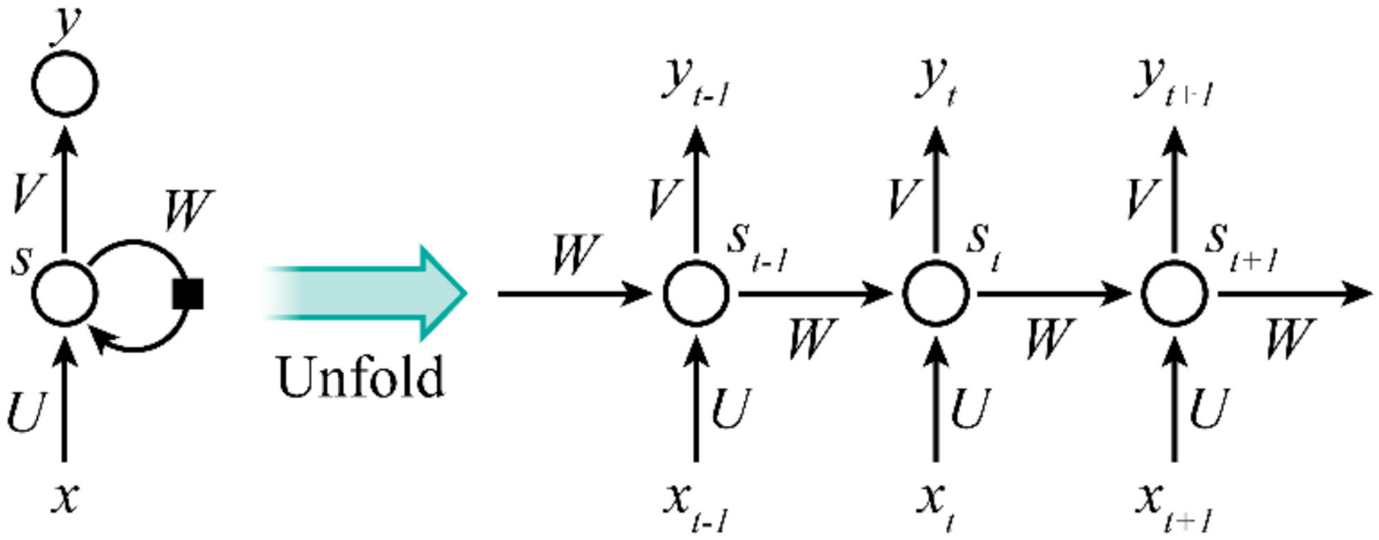
\includegraphics[width=0.8\linewidth]{images/RNN.png}
        \vspace{0pt}
    \caption{Mô hình RNN chuẩn (Nguồn: \cite{DeepLearning})}
    \label{fig7}
    \end{minipage}
\end{figure}
Trạng thái ẩn \( S_t \) tại bước \( t \) được tính dựa trên đầu vào  \( X_t \) tại bước \( t \) và trạng thái ẩn \( S_{t-1} \) tại bước trước:
\[s_{t} = f(U_{x_{t}} + W_{s_{t-1}})\]
Trong đó:
\begin{itemize}
    \item \( s_t \): Trạng thái ẩn tại thời điểm \( t \).
    \item \( x_{t} \): Đầu vào tại thời điểm \( t \).
    \item \( s_{t-1} \): Trạng thái ẩn tại thời điểm \( t-1 \).
    \item \( U \): Ma trận trọng số từ đầu vào đến trạng thái ẩn.
    \item \( W \): Ma trận trọng số từ trạng thái ẩn trước đến trạng thái ẩn hiện tại.
    \item \( f \): Hàm kích hoạt (thường là hàm tanh hoặc sigmoid).
\end{itemize}
\begin{center}
    \(y_t = \sigma(V_{s_{t}})\)
\end{center}
Trong đó:
\begin{itemize}
    \item \( y_t \): Đầu ra tại thời điểm \( t \).
    \item \( s_{t} \): Trạng thái ẩn tại thời điểm \( t \).
    \item \( V \): Ma trận trọng số từ trạng thái ẩn đến đầu ra.
    \item $\sigma$: Hàm kích hoạt. 
\end{itemize}

\subsection{GRU}
Kyunghyun Cho giới thiệu GRU vào năm 2014, là một thuật toán dựa trên RNN tương tự như LSTM nhưng có cấu trúc đơn giản hơn. RNN gặp phải vấn đề Vanishing và Exploding Gradient trong quá trình lan truyền ngược qua thời gian (Backpropagation Through Time). GRU giải quyết vấn đề này bằng cách sử dụng hai cổng: cổng cập nhật và cổng đặt lại. Khác với LSTM, GRU không duy trì trạng thái tế bào (cell state) bên trong và tích hợp thông tin từ trạng thái tế bào vào trạng thái ẩn (hidden state) của nó\cite{ComparisonGRU&ARIMA}.
\begin{figure}[H]
    \centering
    \begin{minipage}{0.8\linewidth}
    \centering
        \vspace{0pt}
        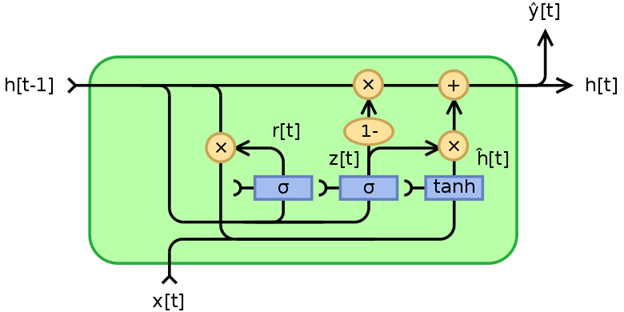
\includegraphics[width=0.8\linewidth]{images/GRU.png}
        \vspace{0pt}
    \caption{Kiến trúc của GRU}
    \label{fig8}
    \end{minipage}
\end{figure}
Reset gate: xác định có bao nhiêu thông tin trong quá khứ phải được giữ lại.
\begin{center}
\(r_t = \sigma(W_r x_t + [h_{t-1}, x_t] + b_r)\)
\end{center}
Update gate: xác định lượng thông tin trước đó sẽ bị xóa và kết hợp đầu vào với thông tin cũ.
\begin{center}
\(z_t = \sigma(W_z x_t + [h_{t-1}, x_t] + b_z)\)
\end{center}
Candidate hidden state: được Reset gate sử dụng để giữ lại thông tin quan trọng từ quá khứ.
\begin{center}
\(\tilde{h}_t = \tanh(W_h [r_t \odot h_{t-1}, x_t] + b_h)\)
\end{center}
Hidden state: là đầu ra của quá trình.
\begin{center}
\(h_t = (1 - z_t) * h_{t-1} + z_t * \tilde{h}_t\)
\end{center}
Trong đó:
\begin{itemize}
    \item $W_r, W_z, W_h$ là những ma trận trọng số.
    \item $x_t$ là đầu vào tại bước thời gian t.
    \item $h_{t-1}$ là trạng thái ẩn trước đó.
    \item $h_t$ là trạng thái ẩn hiện tại.
\end{itemize}


\subsection{LSTM}
LSTM (Long short-term memory) là một phiên bản cải tiến của RNN có một cấu trúc phức tạp được gọi là ô LSTM (LSTM cell) này trong lớp ẩn (hidden layer) của nó. Khối LSTM có 3 cổng tên là cổng vào (input gate), cổng quên (forget gate) và cổng ra (output gate). Ba cổng này có tác dụng điều khiển các luồng thông tin đi qua các ô cũng như mạng nơron. \cite{LSTM} 
\begin{figure}[H]
    \centering
    \begin{minipage}{0.8\linewidth}
    \centering
        \vspace{0pt}
        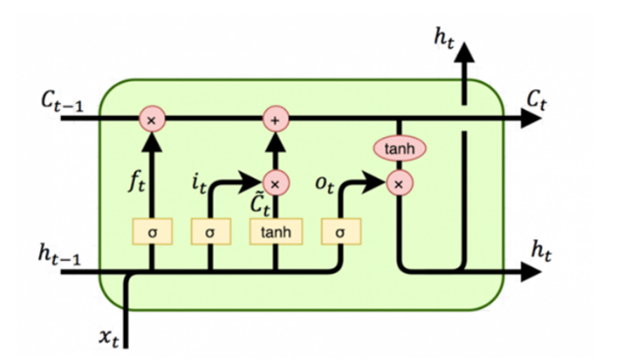
\includegraphics[width=0.8\linewidth]{images/LSTM.png}
        \vspace{0pt}
    \caption{Kiến trúc của LSTM}
    \label{fig9}
    \end{minipage}
\end{figure}
Kiến trúc LSTM cần truyền trạng thái ra của ô $C_t$ (cell output state) và đầu ra lớp ẩn $h_t$ (hidden layer output) tới các nơron tiếp theo trong mạng. Để tính các giá trị này tại thời điểm t ta thực hiện các bước theo thứ tự: \\
\textbf{Bước 1:} Tính trạng thái của 3 cổng, trạng thái đầu vào của ô:
\begin{itemize}
    \item Input gate:
    \(
    i_t = \sigma\left(W_1^i \cdot x_t + W_h^i \cdot h_{t-1} + b_i\right)
    \)
    \item Forget gate:
    \(f_t = \sigma\left(W_1^f \cdot x_t + W_h^f \cdot h_{t-1} + b_f\right)\)
    \item Output gate:
    \(o_t = \sigma\left(W_1^o \cdot x_t + W_h^o \cdot h_{t-1} + b_o\right)\)
    \item Đầu vào của ô:
    \(\tilde{C}_t = \tanh\left(W_1^C \cdot x_t + W_h^C \cdot h_{t-1} + b_C\right)\)
\end{itemize}
Trong đó: 
\begin{itemize}
    \item $x_t$ là dữ liệu đầu vào tại thời điểm $t$
    \item $h_t$ là đầu ra của lớp ẩn, $h_{t-1}$ là đầu ra của trước đó
    \item $\tilde{C}_t$ là trạng thái đầu vào của ô
    \item $W_1^i, W_1^f, W_1^o, W_1^C$ là các ma trận trọng số để kết nối $x_t$ tới 3 cổng và đầu vào của ô
    \item $W_h^i, W_h^f, W_h^o, W_h^C$ là các ma trận trọng số để kết nối $h_{t-1}$ tới 3 cổng và đầu vào của ô
    \item $b_i, b_f, b_o, b_C$ là các chỉ số bias
    \item $\sigma$ là hàm sigmoid với $\sigma = \frac{1}{1 + \exp(-x)}$
    \item $\tanh$ là hàm hyperbolic tangent với $\tanh = \frac{\exp(x) - \exp(-x)}{\exp(x) + \exp(-x)}$
\end{itemize}
\textbf{Bước 2:} Tính toán trạng thái đầu ra của ô:
\[C_t = i_t \cdot \tilde{C}_t + f_t \cdot C_{t-1}\]
Trong đó: 
\begin{itemize}
    \item $C_t$ là trạng thái đầu ra của ô
    \item $C_(t-1)$ là trạng thái đầu ra của trước đó
\end{itemize}
\textbf{Bước 3:} Tính toán đầu ra của lớp ẩn:
\[h_t = o_t \cdot \tanh(C_t)\]

\subsection{CNN-LSTM}
CNN-LSTM (Convolutional Neural Network - Long Short-Term Memory) kết hợp hai kiến trúc mạng nơ-ron quan trọng trong lĩnh vực xử lý dữ liệu hình ảnh và chuỗi. \cite{predictStockCNNLSTM} \\
CNN-LSTM gồm 2 phần là CNN và LSTM:
\subsubsection{Convolutional Neural Network (CNN)} \\
Convolutional Neural Network (CNNs – Mạng nơ-ron tích
chập) là một loại mạng nơron đặc biệt để xử lý dữ liệu có cấu trúc dạng lưới-ma trận. Có 3 loại CNN: 1D CNNs dùng trên dữ liệu chuỗi thời gian, 2D CNNs dùng để phân loại hình ảnh, 3D CNNs thường dùng trong xử lý ảnh 3 chiều hoặc video. 
Một số lớp cơ bản của CNN: 
\begin{itemize}
    \item Convolutional layer: sử dụng các filter để thực hiện phép tích chập. Các siêu tham số của các filter này bao gồm kích thước bộ lọc F (filter) và độ trượt S (stride). Output của convolutional layer sẽ qua hàm activation function trước khi trở thành input của convolutional layer tiếp theo. 
    \item Pooling layer: thường được dùng giữa các lớp Convolutional layer để giảm kích thước dữ liệu nhưng vẫn giữ được các thuộc tính quan trọng. Việc giảm kích thước dữ liệu giúp giảm tính toán trong mô hình. Có 2 loại Pooling Layer phổ biến là: Max Pooling và Average Pooling.
    \item Fully connected layer: Sau khi dữ liệu được truyền qua nhiều convolutional layer và pooling layer thì model đã học được tương đối các đặc điểm của dữ liệu. Fully connected layer nhận đầu vào là các dữ liệu đã được làm phẳng mà mỗi node trong hidden layer được kết nối với tất cả các node trong layer trước. 
\end{itemize}

\subsubsection{Long Short-Term Memory (LSTM)}\\
Đã được nhắc đến trong mục LSTM bên trên.

\subsubsection{Kiến trúc mô hình CNN-LSTM} \\
Kiến trúc CNN-LSTM liên quan đến việc sử dụng các lớp CNN để trích xuất các đặc trưng cục bộ từ dữ liệu đầu vào, sau đó đưa các đặc trưng vào các lớp LSTM để mô hình có thể hiểu các mối quan hệ không gian và thời gian giữa các đặc trưng này. \cite{predictStockCNNLSTM}.

\begin{figure}[H]
    \centering
    \begin{minipage}{0.8\linewidth}
    \centering
        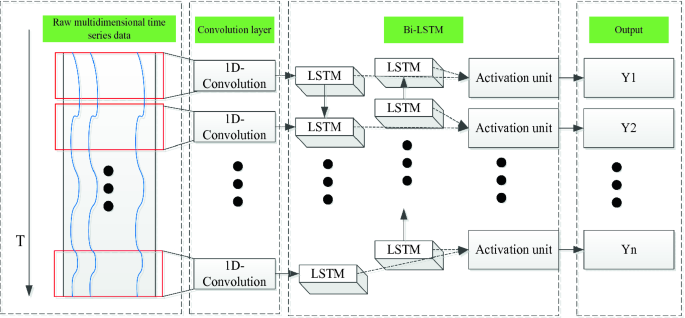
\includegraphics[width=0.8\linewidth]{images/CNNLSTM.png}
    \caption{Kiến trúc của CNN-LSTM (Nguồn: \cite{CNNLSTMTimeSeries})}
    \label{fig10}
    \end{minipage}
\end{figure}
Kiến trúc mô hình CNN-LSTM bao gồm các thành phần sau:
\begin{itemize}
    \item Input Layer: Nhận dữ liệu đầu vào, ví dụ giá đóng cửa, giá sàn,...
    \item CNN Layer: Sử dụng các lớp tích chập để trích xuất đặc trưng giúp mô hình học được những đặc trưng quan trọng cho dự đoán giá cổ phiếu.
    \item LSTM Layer: Nhận các đặc trưng đã được trích xuất từ CNN và sử dụng các memory cell để xử lý và mô hình hóa dữ liệu chuỗi. LSTM giúp mô hình ghi nhớ thông tin lịch sử quan trọng và dự đoán dựa trên quá khứ.
    \item Output Layer: Tạo ra dự đoán về giá cổ phiếu dựa trên trạng thái ẩn cuối cùng của mô hình.
\end{itemize}


\subsection{MICN}
MICN (Multi-Scale Isometric Convolution Network) là mô hình giúp dự đoán hiệu quả và tiết kiệm chi phí cho dự đoán dài hạn bằng cách sử dụng phương pháp tách nhỏ đầu vào và chọn các thuật toán thích hợp để xử lý từ phần nhỏ. Kiến trúc tổng quan của mô hình MICN được thể hiện như sau: \cite{MICN}
\begin{figure}[H]
    \centering
    \begin{minipage}{0.8\linewidth}
    \centering
        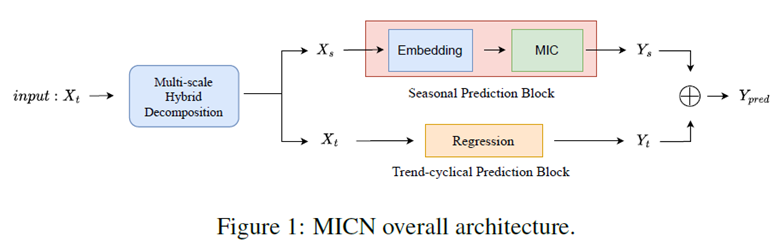
\includegraphics[width=\linewidth]{images/MICN.png}
    \caption{Kiến trúc của MICN}
    \label{fig11}
    \end{minipage}
\end{figure}
Mô hình bao gồm 3 phần chính: một khối phân rã đa tầng kết hợp (Multi-scale hybrid decomposition – MHDecomp), một khối dự đoán cho dữ liệu có tính mùa vụ, một khối dự đoán có dữ liệu có tính xu hướng theo chu kỳ. Sau khi xử lý từng phần xong mô hình sẽ kết hợp kết quả của 2 quá trình lại để cho ra kết quả cuối cùng.

\subsubsection{MULTI-SCALE HYBRID DECOMPOSITION}
Khối phân rã đã tầng kết hợp được xây dựng dựa theo thuật toán phân rã của Haixu Wu là áp dụng trung bình trượt để làm mượt các biến động nhỏ và làm nổi bật các xu hướng dài hạn. Tuy nhiên thuật toán này có điểm yếu khi sử dụng tham số kernel nên ở mô hình MICN đã cải tiến bằng cách sử dụng nhiều kernel khác nhau kết hợp với việc sử dụng giá trị trung bình để xử lý. Với dữ liệu đầu vào là \( X \in \mathbb{R}^{I \times d} \), quá trình phân rã được xử lý như sau:
\resizebox{\linewidth}{!}{
        $X_t = \text{AvgPool(Padding}(X))_{\text{kernel}_1}, \ldots, \text{AvgPool(Padding}(X))_{\text{kernel}_n}$
    }
Trong đó:
\begin{itemize}
    \item \( X_t \) là phần dữ liệu có xu hướng chu kỳ.
    \item \( X_s \) là phần dữ liệu có tính mùa vụ.
\end{itemize}

\subsubsection{TREND-CYCLICAL PREDICTION BLOCK}
Mô hình MICN sử dụng thuật toán hồi quy tuyến tính đơn giản để dự đoán cho dữ liệu có xu hướng theo chu kỳ. Cụ thể với dữ liệu có tính xu hướng theo chu kỳ được xử lý bằng cách:
\[Y{\substack{\text{regre}\\t}}{} = regression(X_t)\]
Trong đó \(Y_{\text{regre}t} \in \mathbb{R}^{O \times d}\) là kết quả dự đoán của phần này dựa trên thuật toán hồi quy tuyến tính.

\subsubsection{SEASONAL PREDICTION BLOCK}
Khối dự đoán cho dữ liệu có tính mùa vụ tập trung vào việc xử lý phần dữ liệu có tính mùa vụ phức tạp. Đầu tiên thực hiện quá trình Embedding chuỗi đầu vào $X_s$, thuật toán tiếp tục áp dụng “Multi-scale isometric convolution” (MIC) để lấy ra những đặc trưng cục bộ và tương quan toàn thể, và các nhánh với các tỷ lệ khác nhau, tức là các mạng con hoặc các tham số khác nhau được sử dụng để mô hình hóa các mẫu cơ bản khác nhau trong chuỗi thời gian. Mỗi nhánh có thể tập trung vào việc xác định mẫu ở một mức độ chi tiết khác nhau. Cuối cùng kết hợp các kết quả từ các nhánh khác nhau để hoàn thiện việc sử dụng thông tin toàn diện của chuỗi.
\begin{figure}[H]
    \centering
    \begin{minipage}{0.8\linewidth}
    \centering
        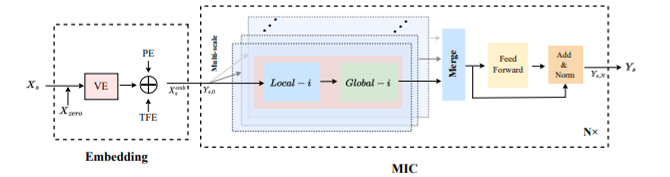
\includegraphics[width=\linewidth]{images/MICN_SeasonalBlock.png}
    \caption{Khối dự đoán dữ liệu mùa vụ}
    \label{fig11}
    \end{minipage}
\end{figure}
\begin{figure}[H]
    \centering
    \begin{minipage}{0.8\linewidth}
    \centering
        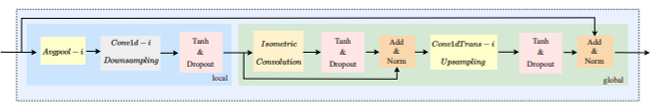
\includegraphics[width=\linewidth]{images/MICN_LocalGlobalModule.png}
    \caption{Kiến trúc module cục bộ-toàn cầu}
    \label{fig11}
    \end{minipage}
\end{figure}
Các quá trình được tổng kết lại bằng các công thức sau:
\begin{center}
\(X{\substack{\text{emb}\\s}}{} = {\text{Embedding}}(\text{Concat}(X_s, X_{\text{zero}}))\) \\
\(Y{\substack{\text{0}\\s}}{} = X{\substack{\text{emb}\\s}}{}\)\\
\(Y_{s,l} = \text{MIC}(Y_{s,l-1}), \quad l \in \{1, 2, \ldots, N\}\)\\
\(Y_s = \text{Truncate}(\text{Projection}(Y_{s,N}))\)
\end{center}
Trong đó:
\begin{itemize}
    \item \(X_{\text{zero}} \in \mathbb{R}^{O \times d}\): các chỗ trống được điền bằng zero
    \item \(X_{\text{emb}}^s \in \mathbb{R}^{(I+O) \times D}\): các dữ liệu đã được nhúng từ \(X_s\)
    \item \(Y_{s,l} \in \mathbb{R}^{(I+O) \times D}\): kết quả dự đoán của lớp MIC thứ \(l\)
    \item \(Y_s\): kết quả dự đoán cuối cùng cho dữ liệu có tính mùa vụ
\end{itemize}


\section{KẾT QUẢ}
\subsection{CÁC PHƯƠNG PHÁP ĐÁNH GIÁ}
MAPE (Mean Absolute Percentage Error): tính toán sự sai lệch trung bình theo tỷ lệ phần trăm giữa giá trị dự báo và giá trị thực tế. Tuy nhiên khi giá trị thực tế gần bằng 0, MAPE có thể dẫn đến phép chia cho 0 gây sai lệch trong kết quả đánh giá.
\[\text{MAPE} = \frac{1}{n} \sum_{t=1}^{n} \left| \frac{y_i - \hat{y}_i}{y_i} \right| \times 100\%\]
Root Mean Squared Error (RMSE): là độ lệch chuẩn của các phần dư (sai số dự đoán). RMSE được tính bằng cách lấy căn bậc hai của trung bình của bình phương các sai số giữa giá trị dự đoán và giá trị thực tế. Tuy nhiên, RMSE có thể bị ảnh hưởng bởi các giá trị ngoại lai (outliers) trong dữ liệu. 
\[\text{RMSE} = \sqrt{\frac{1}{n} \sum_{i=1}^{n} (y_i - \hat{y}_i)^2}\]

Mean Absolute Error (MAE): dùng để so sánh hiệu suất và đánh giá mức độ chính xác của các mô hình dự báo. MAE đo lường độ lỗi trung bình tuyệt đối giữa giá trị dự đoán và giá trị thực tế. MAE càng nhỏ thì mô hình dự đoán càng chính xác.
\[\text{MAE} = \frac{1}{n} \sum_{i=1}^{n} |y_i - \hat{y}_i|\]

Trong đó:
\begin{itemize}
    \item \(n\): số lượng mẫu
    \item \(y_i\): giá trị thực tế của mẫu thứ \(i\)
    \item \(\hat{y}_i\): giá trị dự đoán tương ứng của mô hình cho mẫu thứ \(i\)
\end{itemize}



\subsection{TRỰC QUAN HÓA}

\subsubsection{ĐÁNH GIÁ TRÊN BỘ DỮ LIỆU BIDV}

\begin{minipage}{0.21\textwidth}
    \centering
    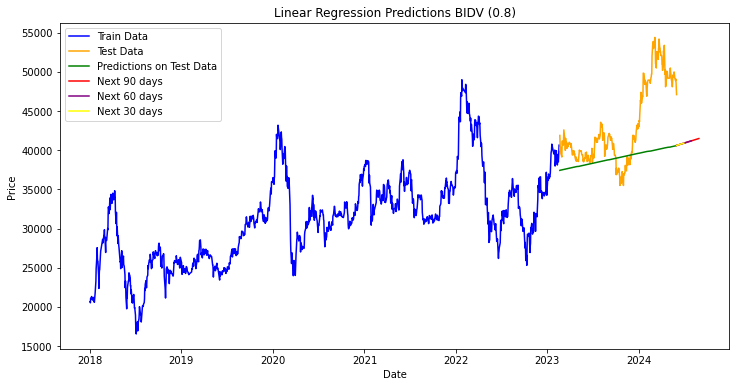
\includegraphics[width=\linewidth]{images/LR/LR_BIDV_82.png}
    \captionof{figure}{LR 8:2}
    \label{fig:image1}
\end{minipage}
\hfill
\begin{minipage}{0.21\textwidth}
    \centering
    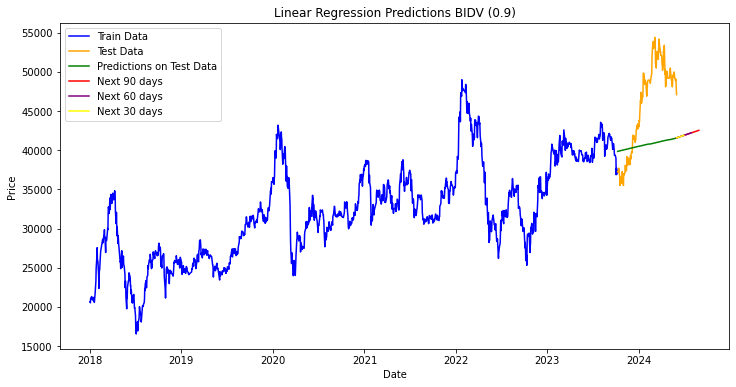
\includegraphics[width=\linewidth]{images/LR/LR_BIDV_91.png}
    \captionof{figure}{LR 9:1}
    \label{fig:image2}
\end{minipage}

\begin{minipage}{0.21\textwidth}
    \centering
    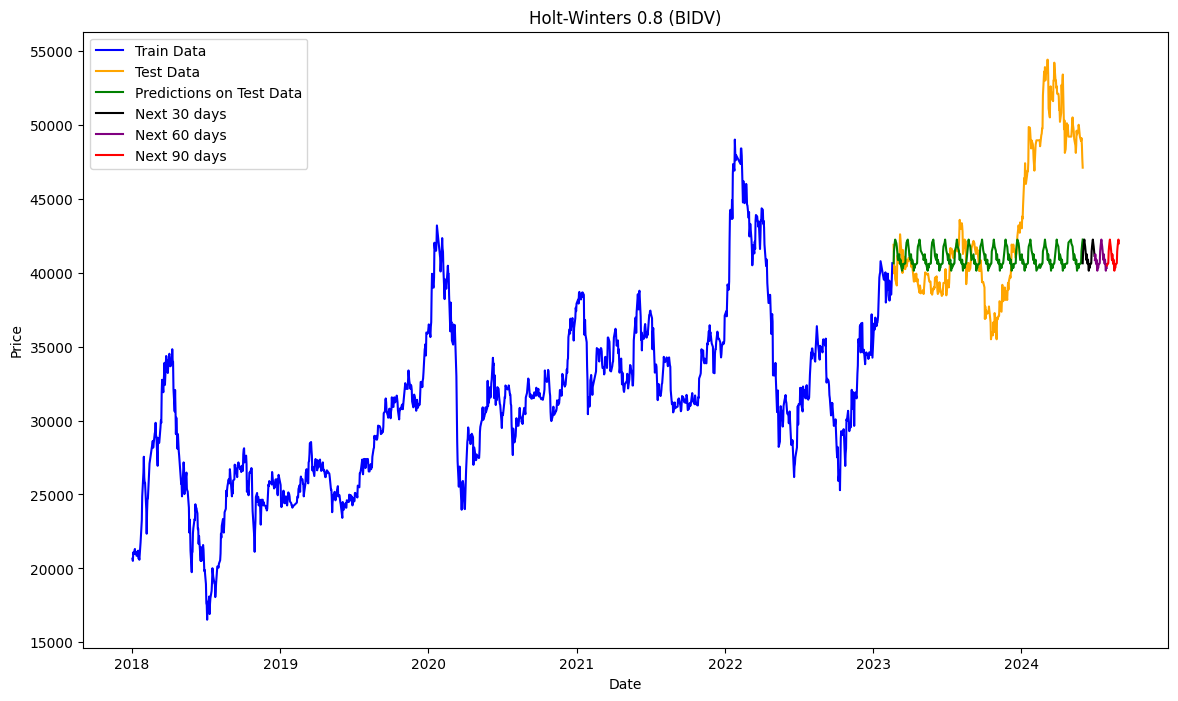
\includegraphics[width=\linewidth]{images/Holt Winter/HW_BIDV_82.png}
    \captionof{figure}{Holt-Winter 8:2}
    \label{fig:image1}
\end{minipage}
\hfill
\begin{minipage}{0.21\textwidth}
    \centering
    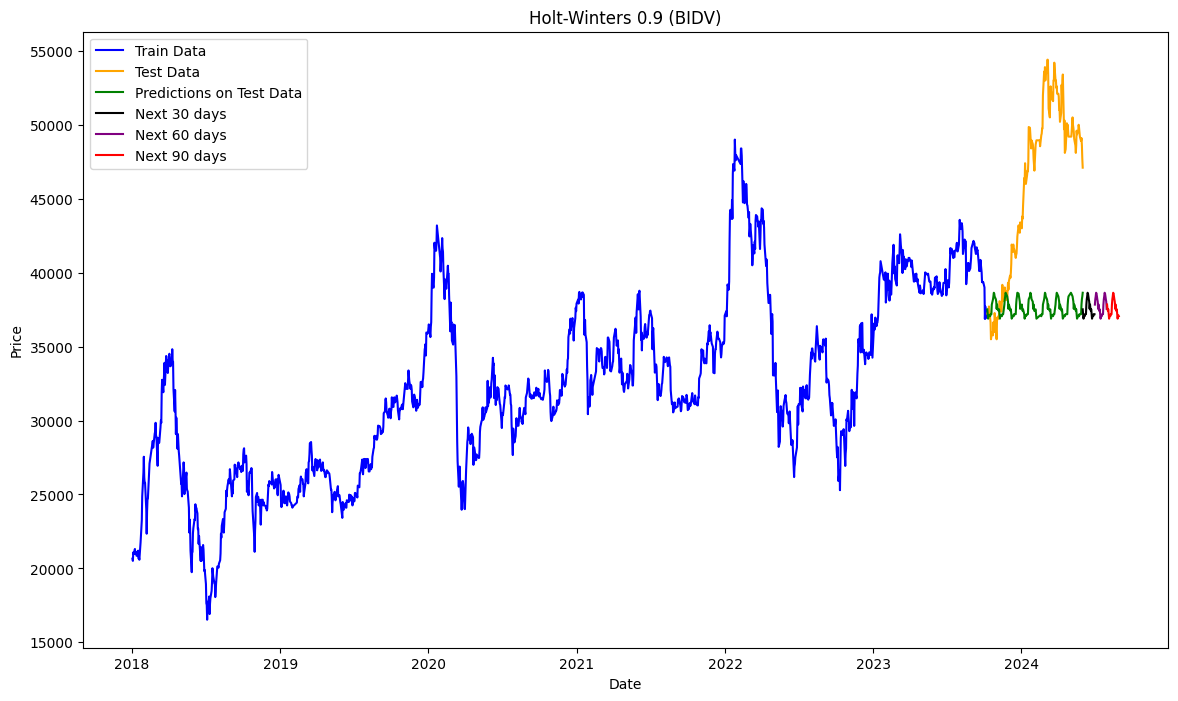
\includegraphics[width=\linewidth]{images/Holt Winter/HW_BIDV_91.png}
    \captionof{figure}{Holt-Winter 9:1}
    \label{fig:image2}
\end{minipage}

\begin{minipage}{0.21\textwidth}
    \centering
    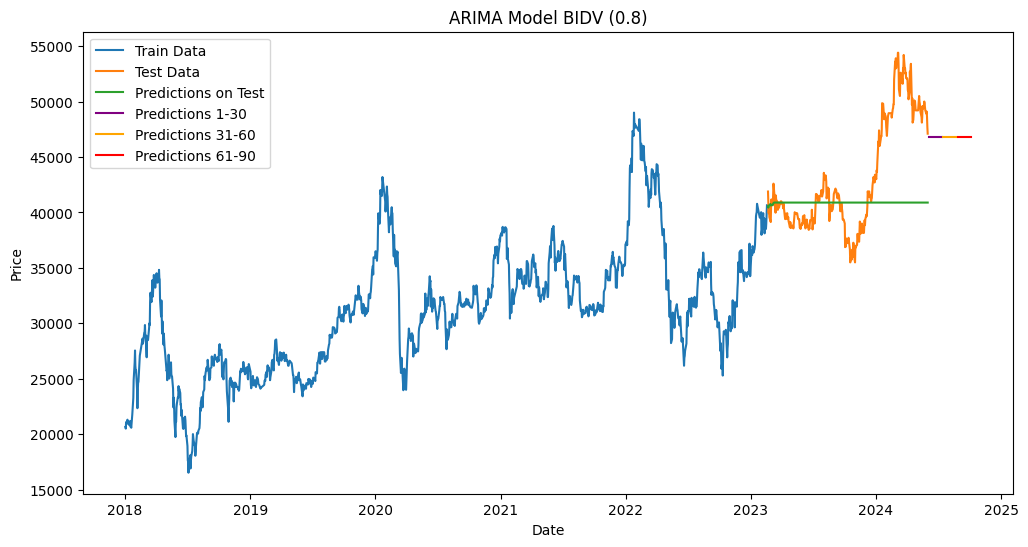
\includegraphics[width=\linewidth]{images/ARIMA/ARIMA_BIDV_82.png}
    \captionof{figure}{ARIMA 8:2 }
    \label{fig:image1}
\end{minipage}
\hfill
\begin{minipage}{0.21\textwidth}
    \centering
    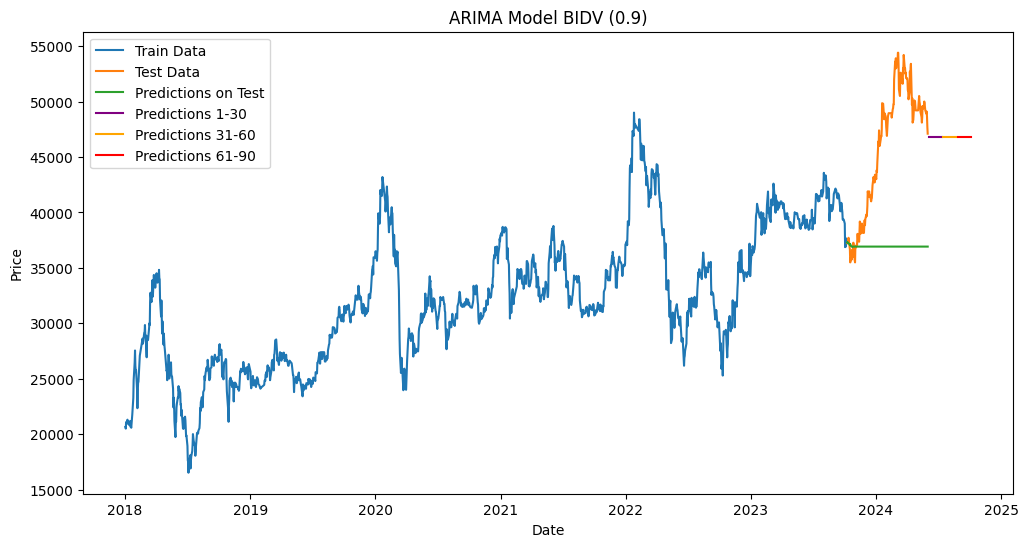
\includegraphics[width=\linewidth]{images/ARIMA/ARIMA_BIDV_91.png}
    \captionof{figure}{ARIMA 9:1 }
    \label{fig:image2}
\end{minipage}

\begin{minipage}{0.21\textwidth}
    \centering
    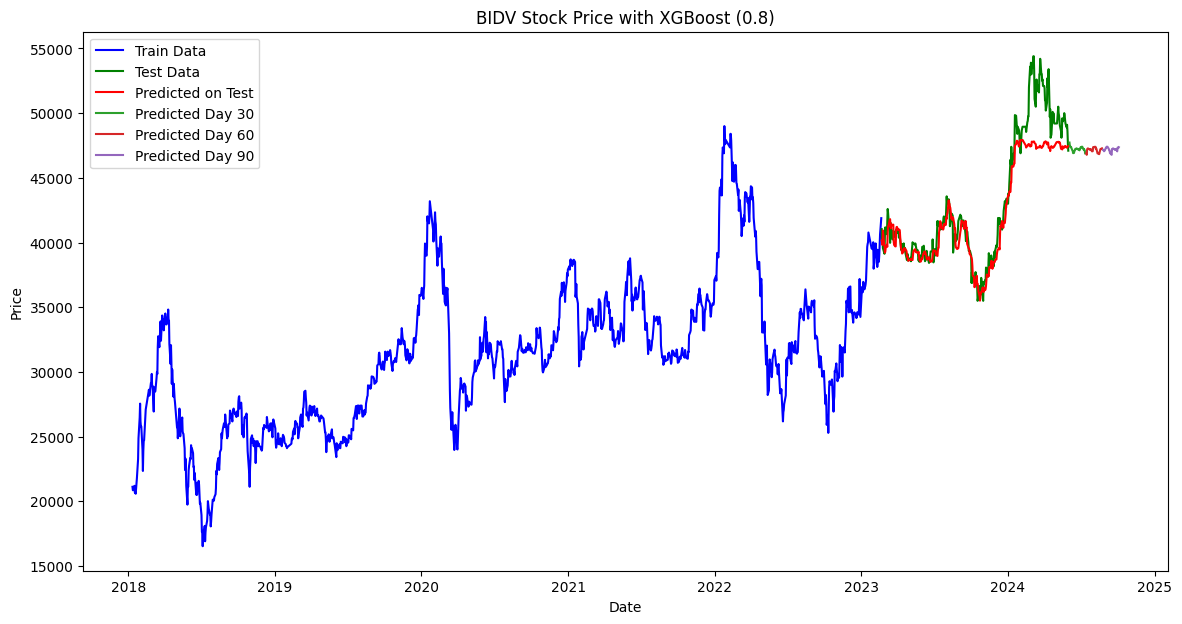
\includegraphics[width=\linewidth]{images/XGBoost/XGBoost_BIDV_82.png}
    \captionof{figure}{XGBoost 8:2 }
    \label{fig:image1}
\end{minipage}
\hfill
\begin{minipage}{0.21\textwidth}
    \centering
    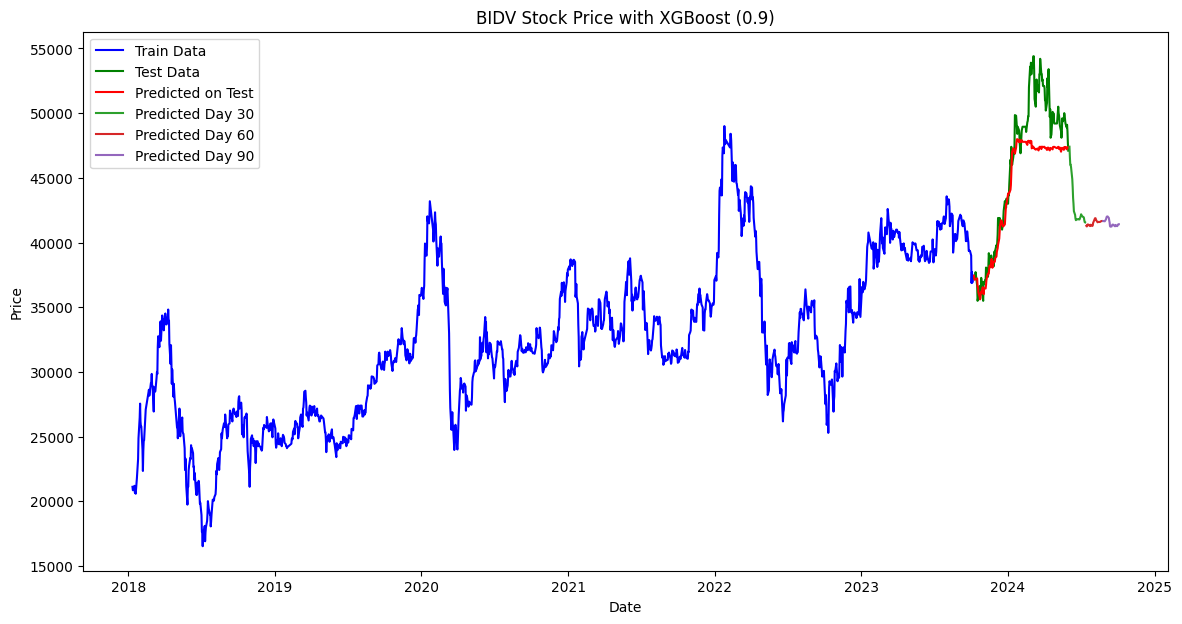
\includegraphics[width=\linewidth]{images/XGBoost/XGBoost_BIDV_91.png}
    \captionof{figure}{XGBoost 9:1 }
    \label{fig:image2}
\end{minipage}

\begin{minipage}{0.21\textwidth}
    \centering
    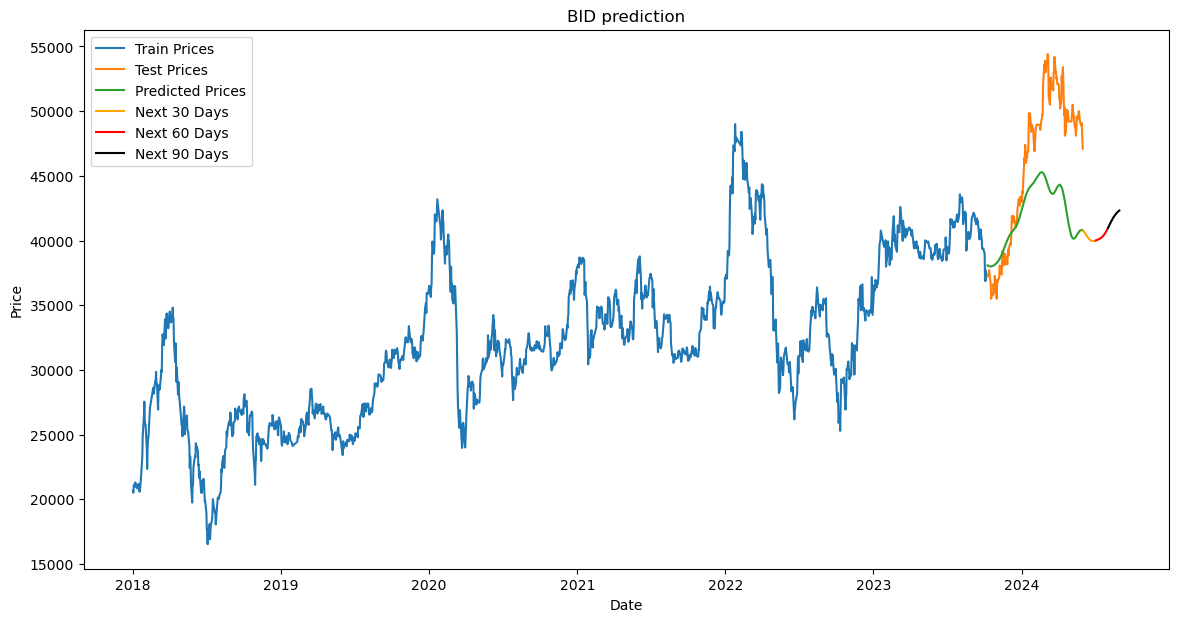
\includegraphics[width=\linewidth]{images/LR CalendarFourier, DeterministicProcess/LRCD_BIDV_91.png}
    \captionof{figure}{Linear Regression CalendarFourier, DeterministicProcess 8:2}
    \label{fig:image1}
\end{minipage}
\hfill
\begin{minipage}{0.21\textwidth}
    \centering
    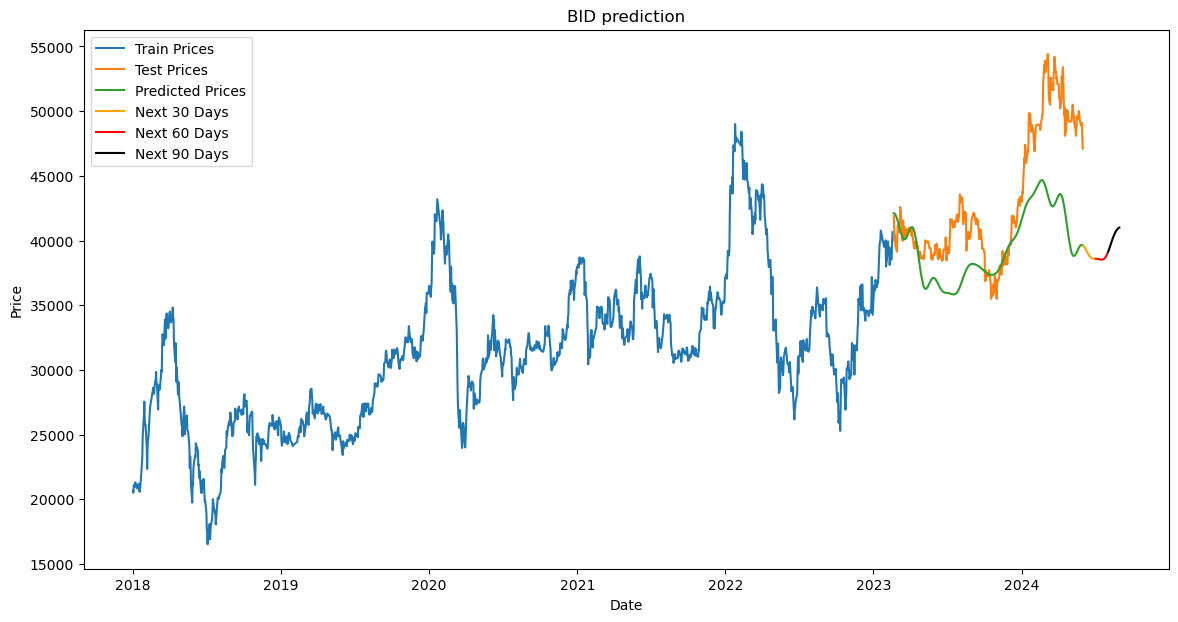
\includegraphics[width=\linewidth]{images/LR CalendarFourier, DeterministicProcess/LRCD_BIDV_82.png}
    \captionof{figure}{Linear Regression CalendarFourier, DeterministicProcess 9:1}
    \label{fig:image2}
\end{minipage}

\begin{minipage}{0.21\textwidth}
    \centering
    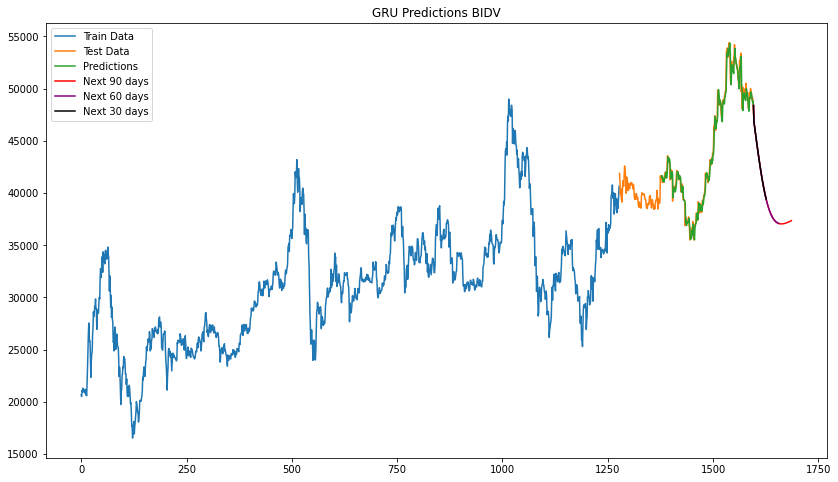
\includegraphics[width=\linewidth]{images/GRU/GRU_BIDV_82.png}
    \captionof{figure}{GRU with 8:2 ratio}
    \label{fig:image1}
\end{minipage}
\hfill
\begin{minipage}{0.21\textwidth}
    \centering
    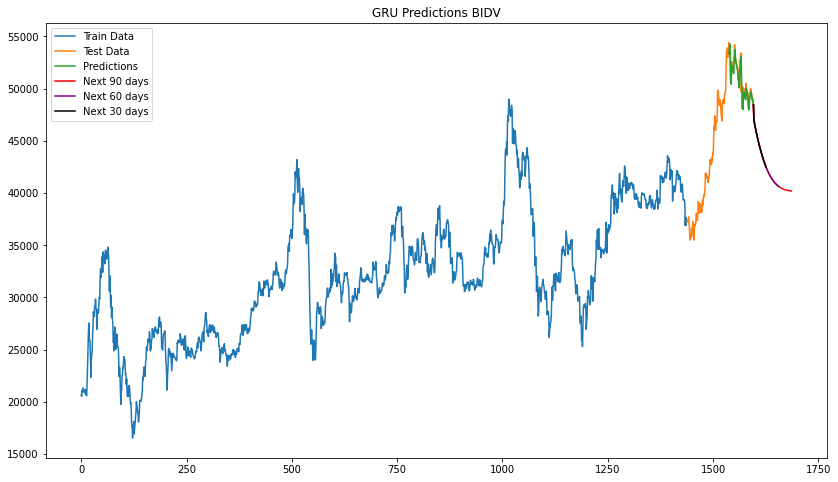
\includegraphics[width=\linewidth]{images/GRU/GRU_BIDV_91.png}
    \captionof{figure}{GRU 9:1 }
    \label{fig:image2}
\end{minipage}

\begin{minipage}{0.21\textwidth}
    \centering
    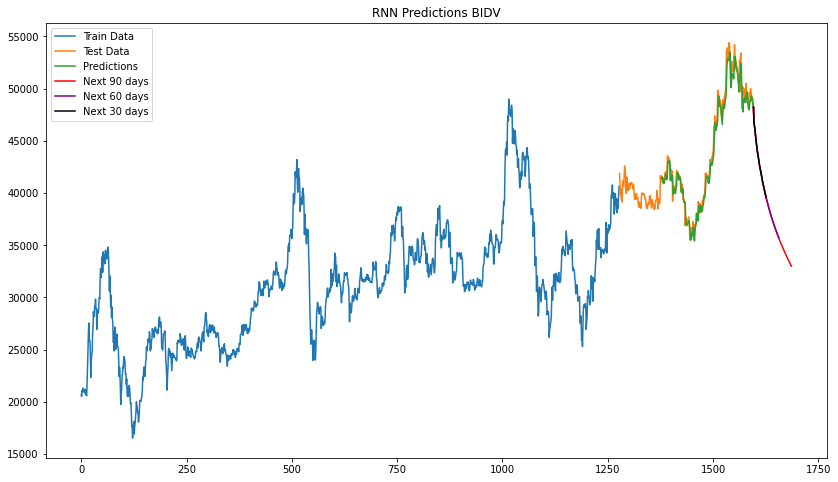
\includegraphics[width=\linewidth]{images/RNN/RNN_BIDV_82.png}
    \captionof{figure}{RNN 8:2 }
    \label{fig:image1}
\end{minipage}
\hfill
\begin{minipage}{0.21\textwidth}
    \centering
    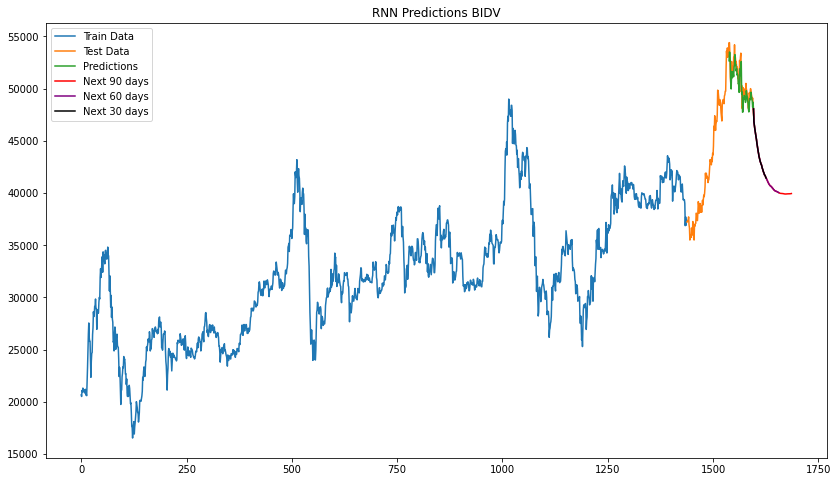
\includegraphics[width=\linewidth]{images/RNN/RNN_BIDV_91.png}
    \captionof{figure}{RNN 9:1}
    \label{fig:image2}
\end{minipage}

\begin{minipage}{0.21\textwidth}
    \centering
    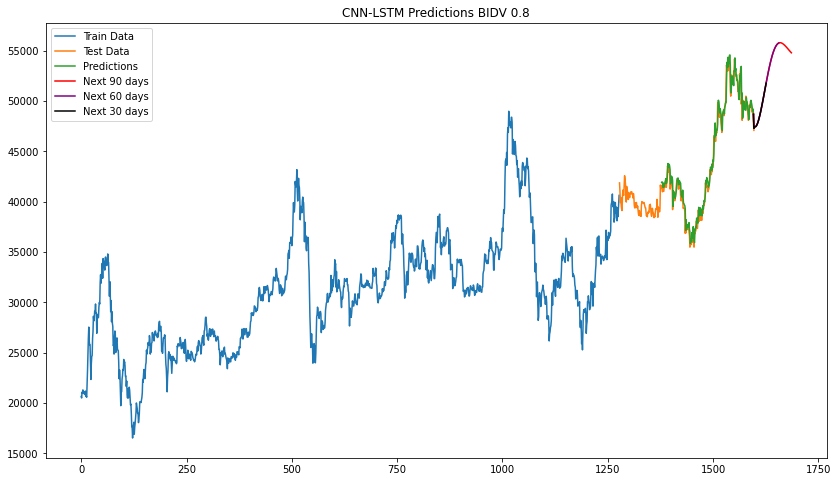
\includegraphics[width=\linewidth]{images/CNN-LSTM/CNNLSTM_BIDV_82.png}
    \captionof{figure}{LSTM 8:2}
    \label{fig:image1}
\end{minipage}
\hfill
\begin{minipage}{0.21\textwidth}
    \centering
    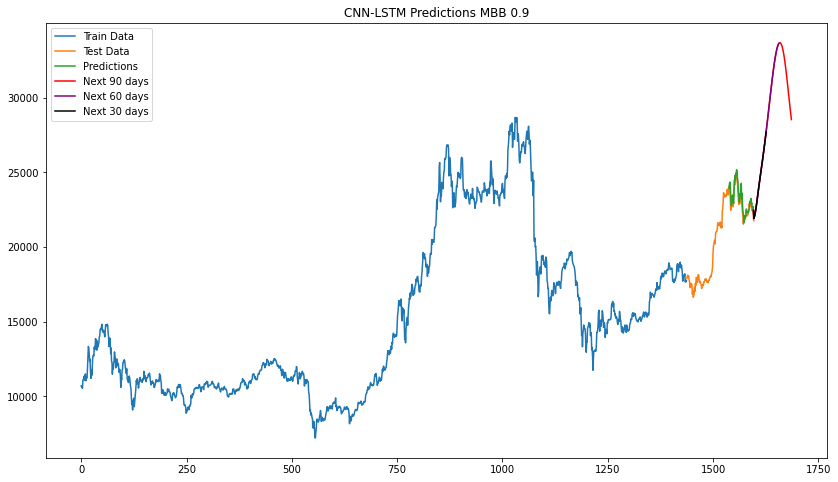
\includegraphics[width=\linewidth]{images/CNN-LSTM/CNNLSTM_BIDV_91.png}
    \captionof{figure}{LSTM 9:1}
    \label{fig:image2}
\end{minipage}

\begin{minipage}{0.21\textwidth}
    \centering
    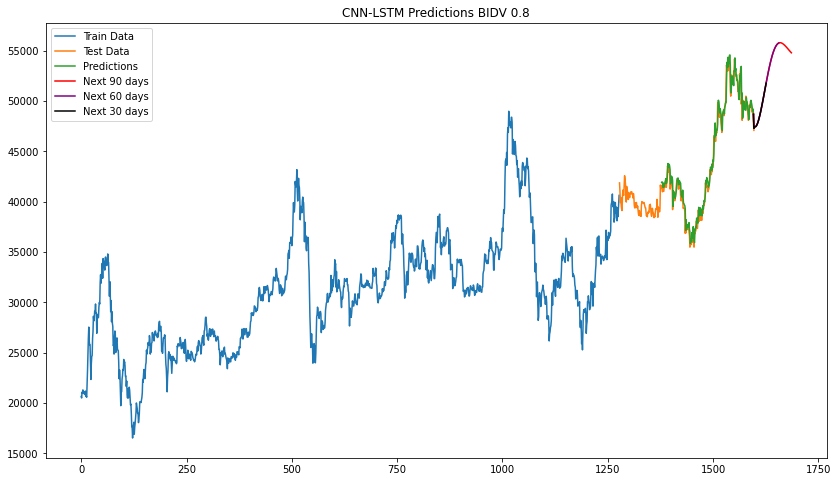
\includegraphics[width=\linewidth]{images/CNN-LSTM/CNNLSTM_BIDV_82.png}
    \captionof{figure}{CNN-LSTM 8:2}
    \label{fig:image1}
\end{minipage}
\hfill
\begin{minipage}{0.21\textwidth}
    \centering
    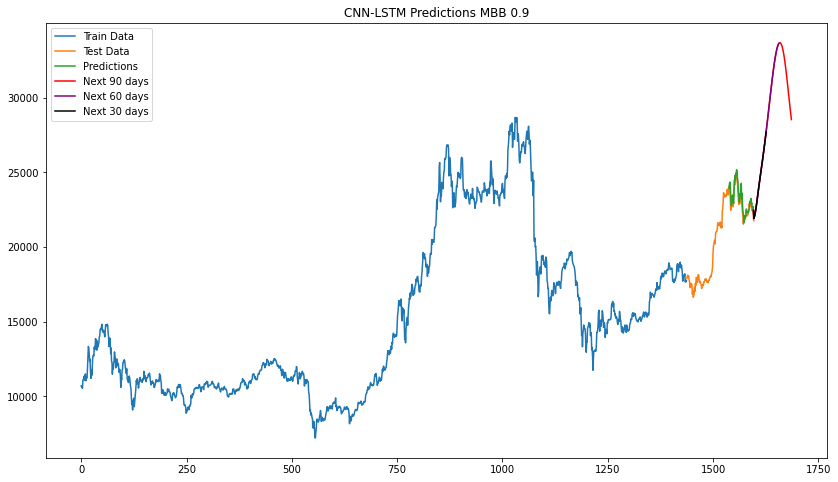
\includegraphics[width=\linewidth]{images/CNN-LSTM/CNNLSTM_BIDV_91.png}
    \captionof{figure}{CNN-LSTM 9:1}
    \label{fig:image2}
\end{minipage}

\begin{minipage}{0.21\textwidth}
    \centering
    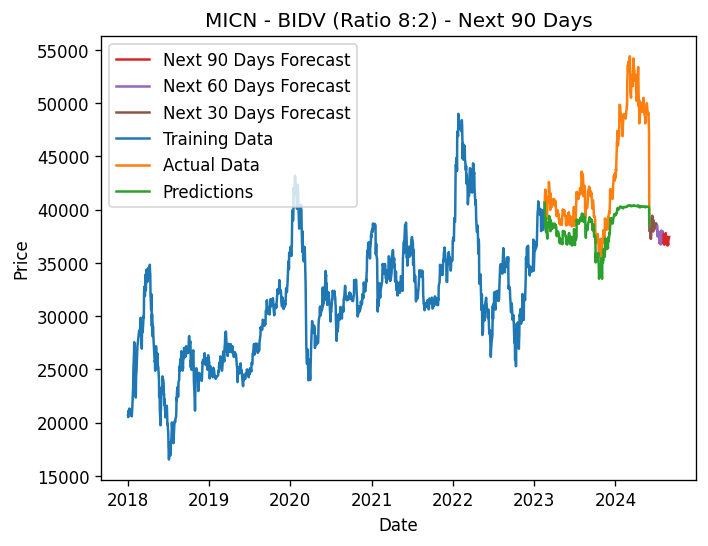
\includegraphics[width=\linewidth]{images/MICN/MICN_BIDV_82.png}
    \captionof{figure}{MICN 8:2 }
    \label{fig:image1}
\end{minipage}
\hfill
\begin{minipage}{0.21\textwidth}
    \centering
    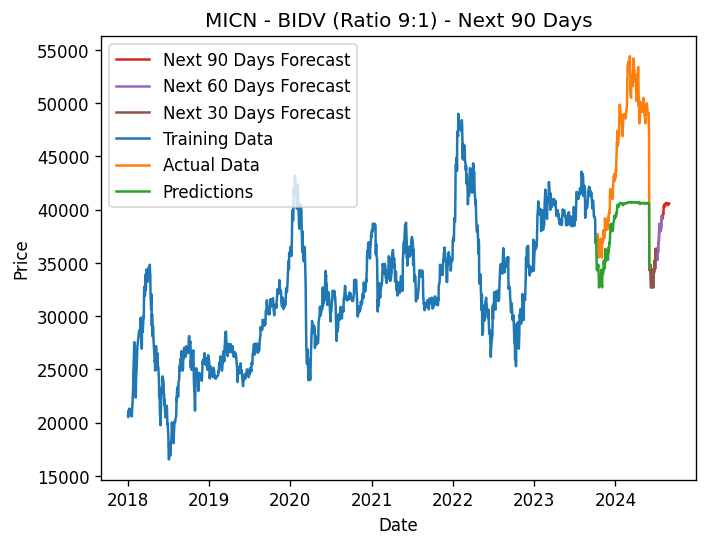
\includegraphics[width=\linewidth]{images/MICN/MICN_BIDV_91.png}
    \captionof{figure}{MICN 9:1 }
    \label{fig:image2}
\end{minipage}

\subsubsection{ĐÁNH GIÁ TRÊN BỘ DỮ LIỆU VCB}
\begin{minipage}{0.21\textwidth}
    \centering
    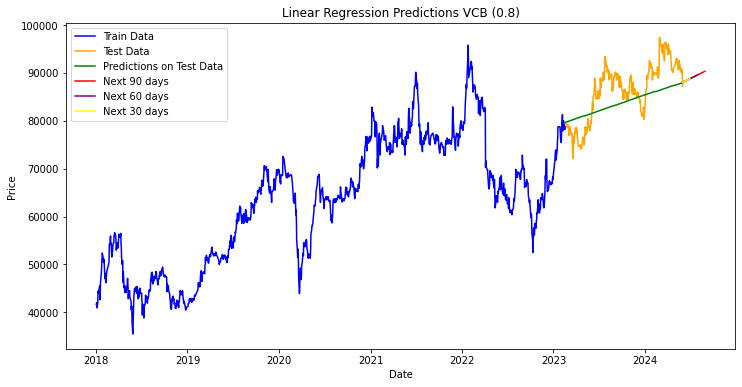
\includegraphics[width=\linewidth]{images/LR/LR_VCB_82.png}
    \captionof{figure}{LR 8:2}
    \label{fig:image1}
\end{minipage}
\hfill
\begin{minipage}{0.21\textwidth}
    \centering
    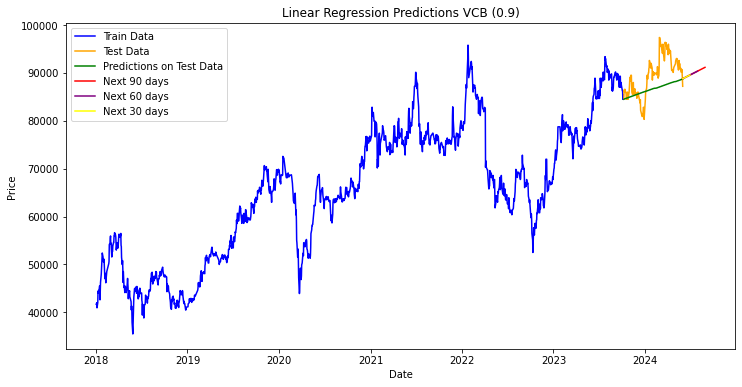
\includegraphics[width=\linewidth]{images/LR/LR_VCB_91.png}
    \captionof{figure}{LR 9:1}
    \label{fig:image2}
\end{minipage}

\begin{minipage}{0.21\textwidth}
    \centering
    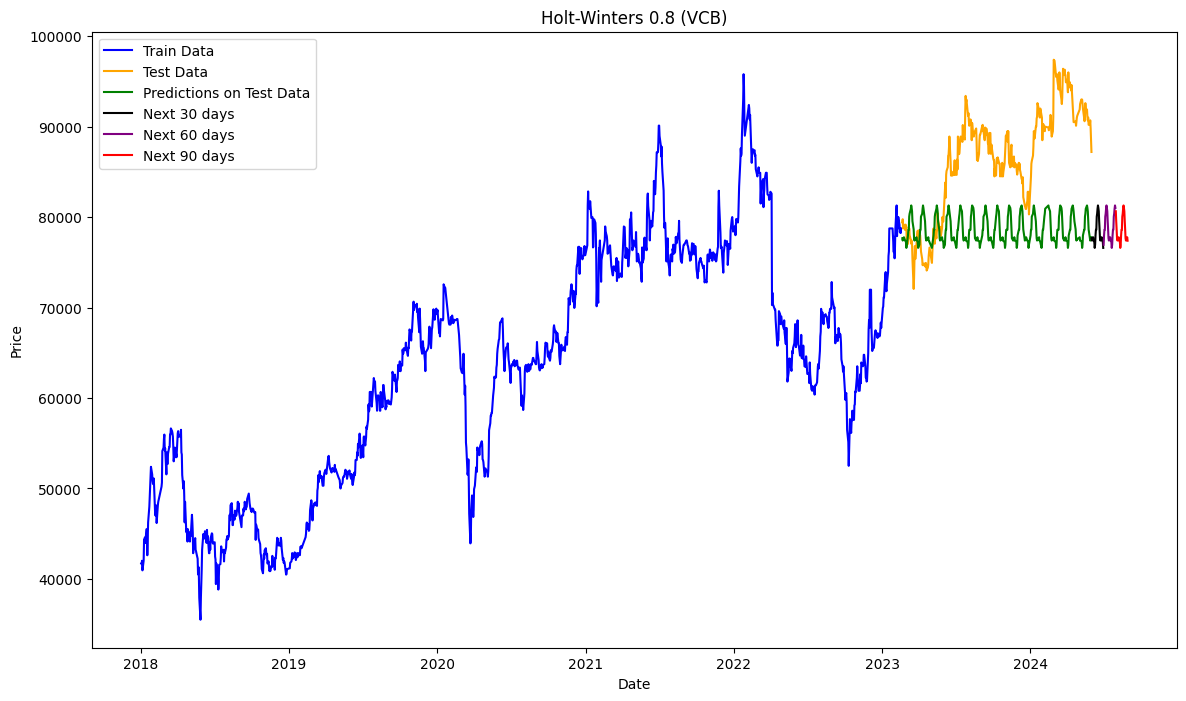
\includegraphics[width=\linewidth]{images/Holt Winter/HW_VCB_82.png}
    \captionof{figure}{Holt-Winter 8:2}
    \label{fig:image1}
\end{minipage}
\hfill
\begin{minipage}{0.21\textwidth}
    \centering
    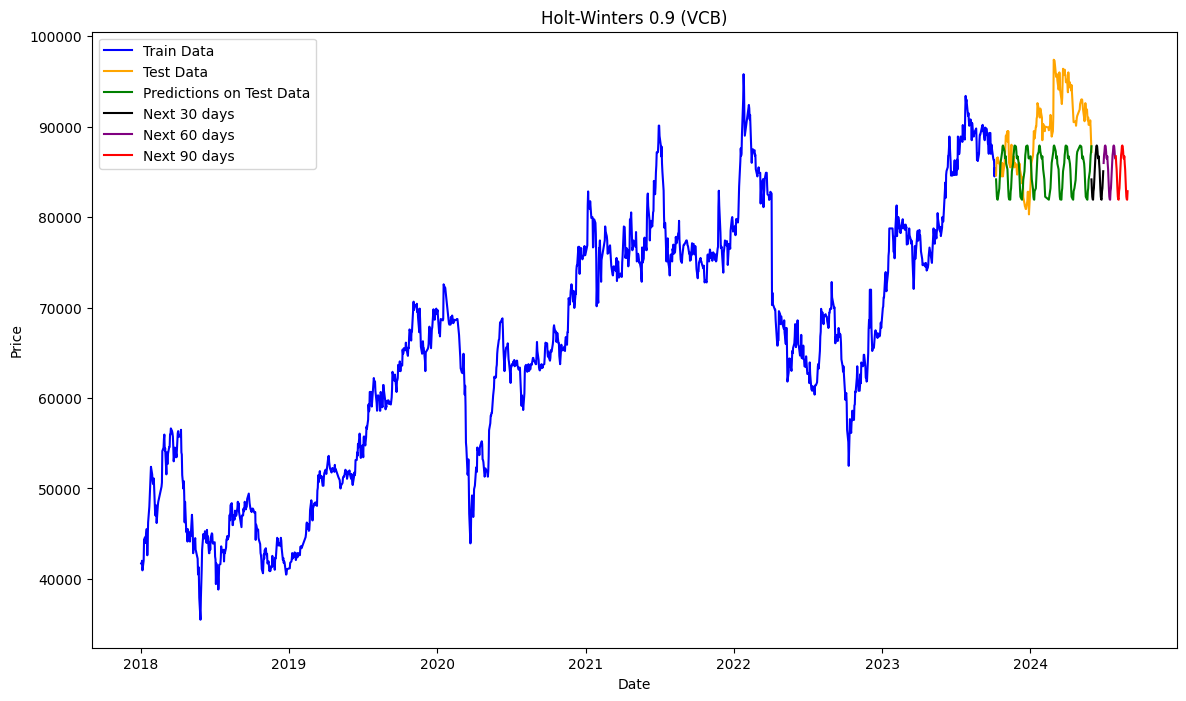
\includegraphics[width=\linewidth]{images/Holt Winter/HW_VCB_91.png}
    \captionof{figure}{Holt-Winter 9:1}
    \label{fig:image2}
\end{minipage}

\begin{minipage}{0.21\textwidth}
    \centering
    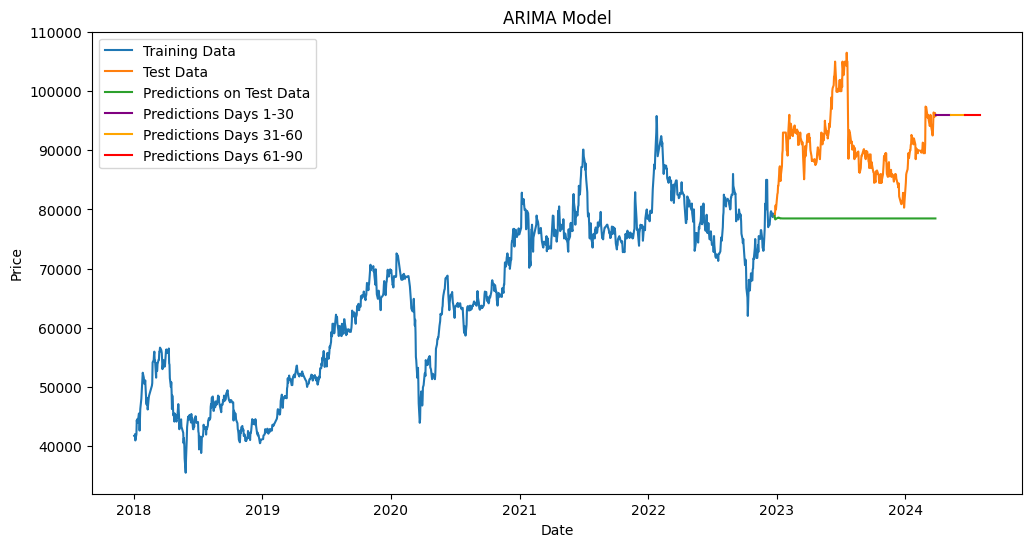
\includegraphics[width=\linewidth]{images/ARIMA/ARIMA_VCB_82.png}
    \captionof{figure}{ARIMA 8:2 }
    \label{fig:image1}
\end{minipage}
\hfill
\begin{minipage}{0.21\textwidth}
    \centering
    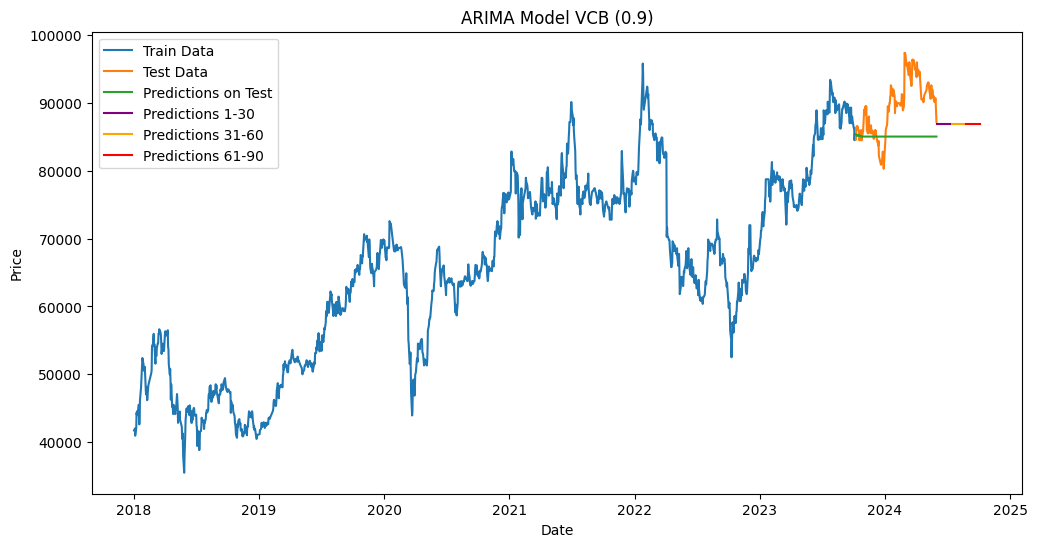
\includegraphics[width=\linewidth]{images/ARIMA/ARIMA_VCB_91.png}
    \captionof{figure}{ARIMA 9:1 }
    \label{fig:image2}
\end{minipage}

\begin{minipage}{0.21\textwidth}
    \centering
    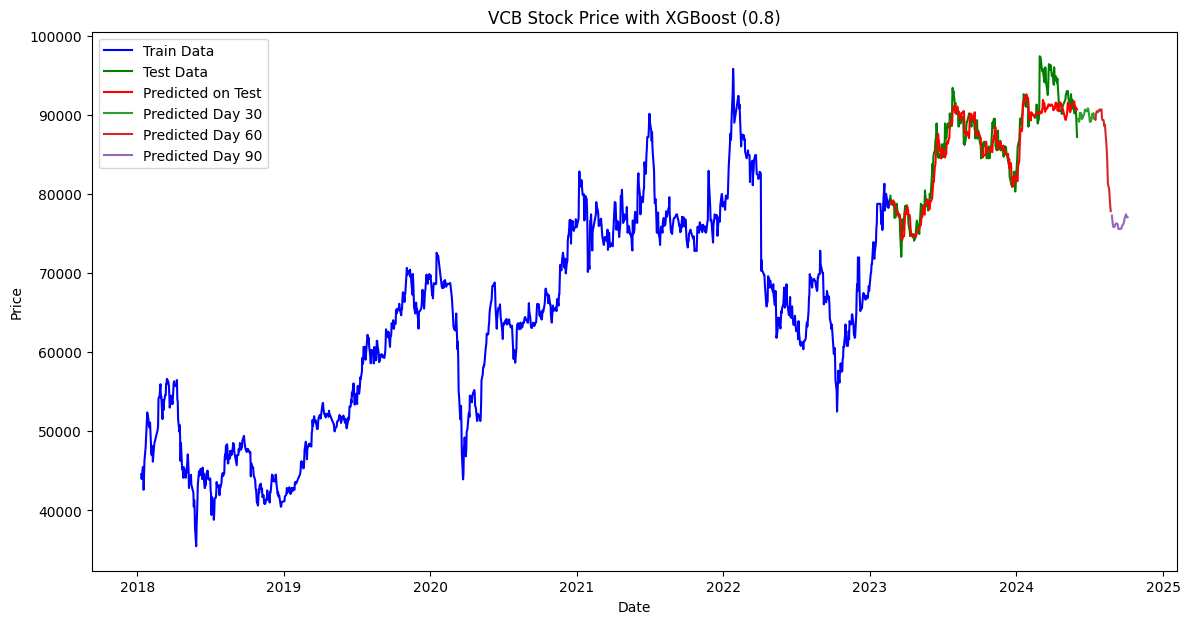
\includegraphics[width=\linewidth]{images/XGBoost/XGBoost_VCB_82.png}
    \captionof{figure}{XGBoost 8:2 }
    \label{fig:image1}
\end{minipage}
\hfill
\begin{minipage}{0.21\textwidth}
    \centering
    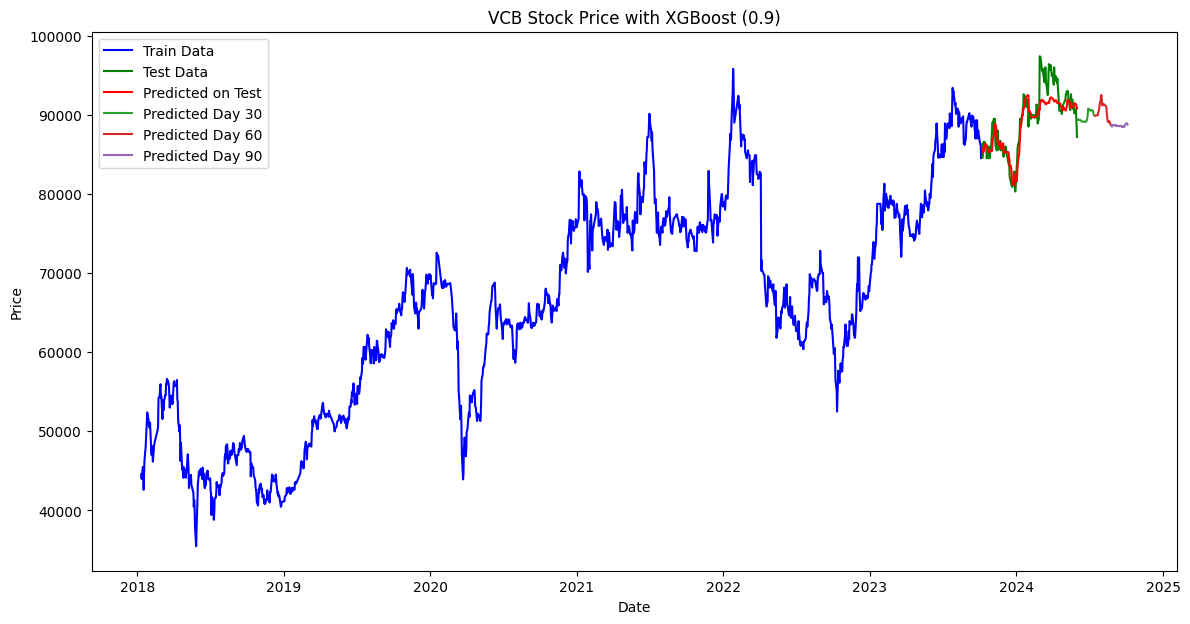
\includegraphics[width=\linewidth]{images/XGBoost/XGBoost_VCB_91.png}
    \captionof{figure}{XGBoost 9:1 }
    \label{fig:image2}
\end{minipage}

\begin{minipage}{0.21\textwidth}
    \centering
    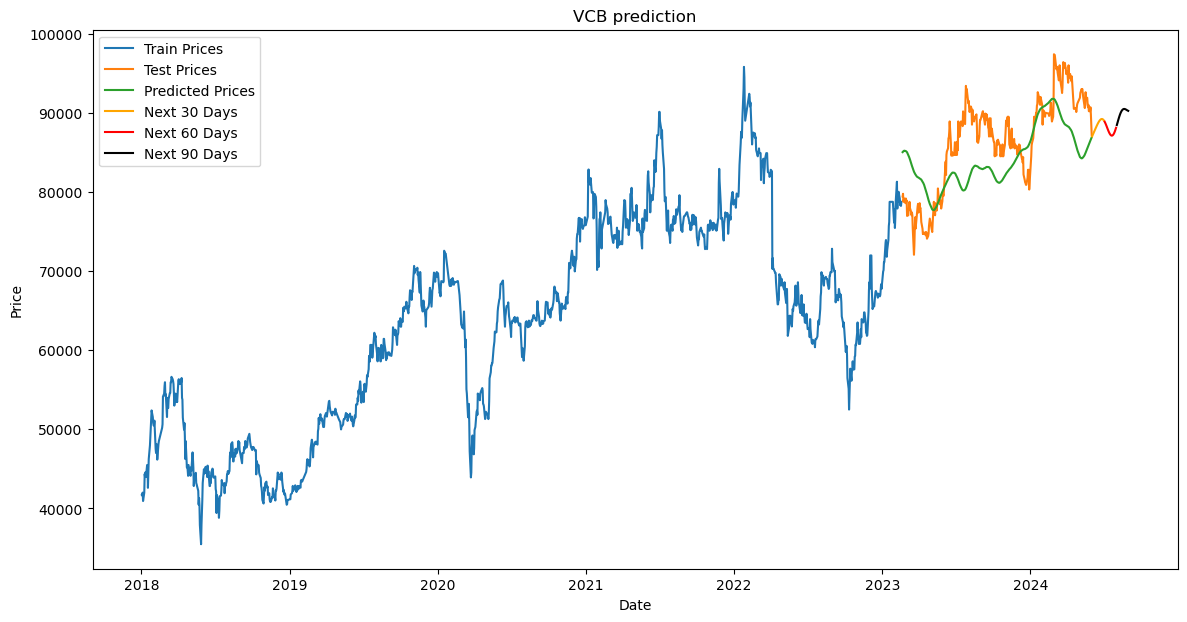
\includegraphics[width=\linewidth]{images/LR CalendarFourier, DeterministicProcess/LRCD_VCB_82.png}
    \captionof{figure}{Linear Regression CalendarFourier, DeterministicProcess 8:2}
    \label{fig:image1}
\end{minipage}
\hfill
\begin{minipage}{0.21\textwidth}
    \centering
    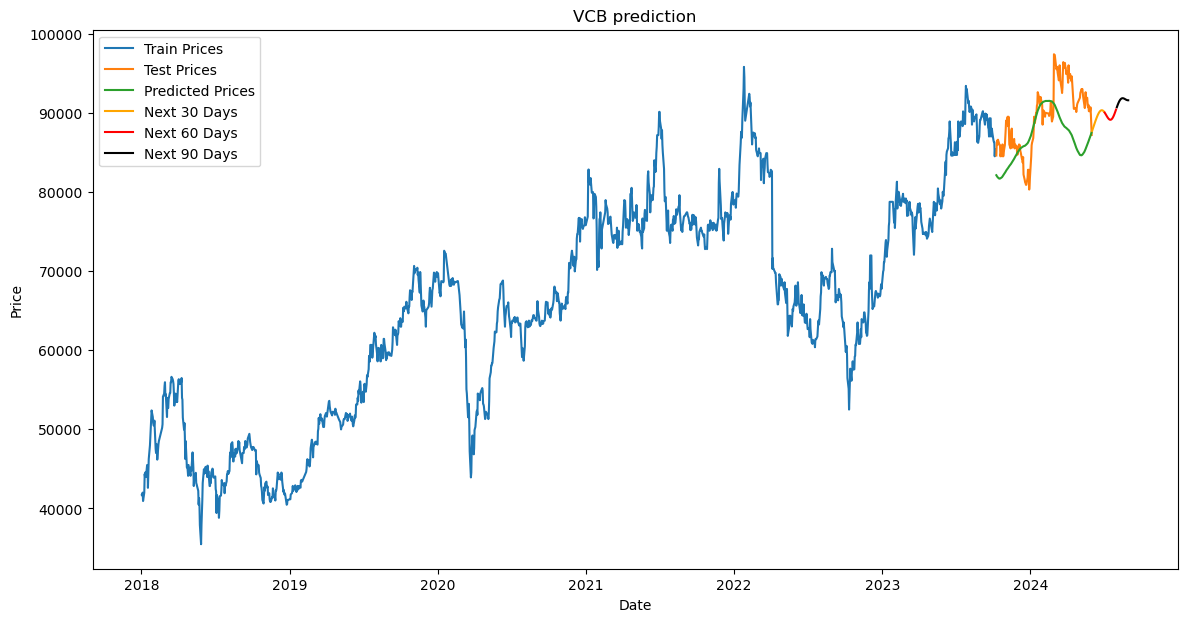
\includegraphics[width=\linewidth]{images/LR CalendarFourier, DeterministicProcess/LRCD_VCB_91.png}}
    \captionof{figure}{Linear Regression CalendarFourier, DeterministicProcess 9:1 }
    \label{fig:image2}
\end{minipage}

\begin{minipage}{0.21\textwidth}
    \centering
    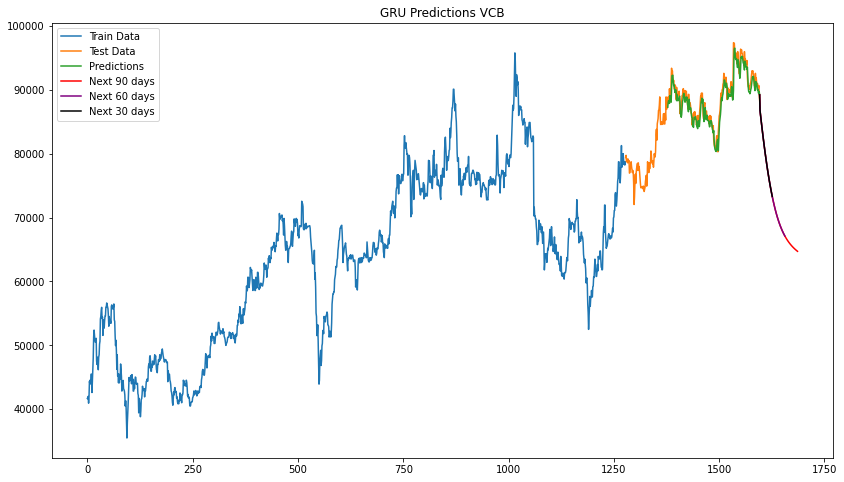
\includegraphics[width=\linewidth]{images/GRU/GRU_VCB_82.png}
    \captionof{figure}{GRU 8:2 }
    \label{fig:image1}
\end{minipage}
\hfill
\begin{minipage}{0.21\textwidth}
    \centering
    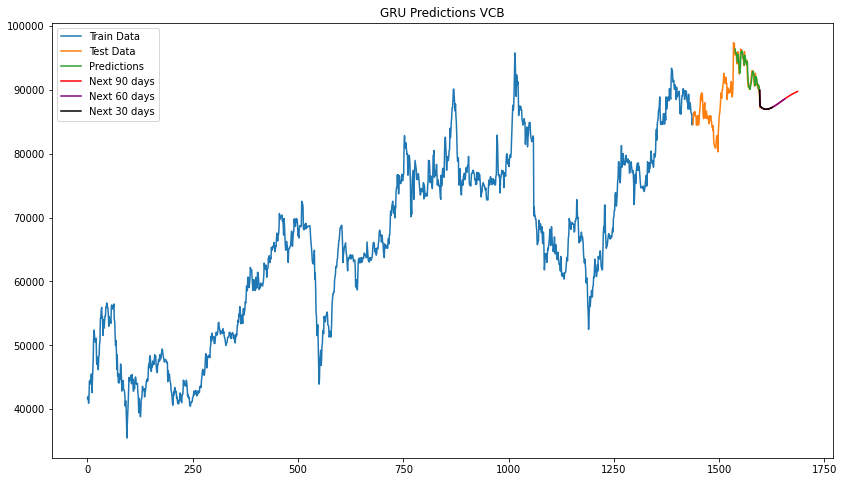
\includegraphics[width=\linewidth]{images/GRU/GRU_VCB_91.png}
    \captionof{figure}{GRU 9:1}
    \label{fig:image2}
\end{minipage}

\begin{minipage}{0.21\textwidth}
    \centering
    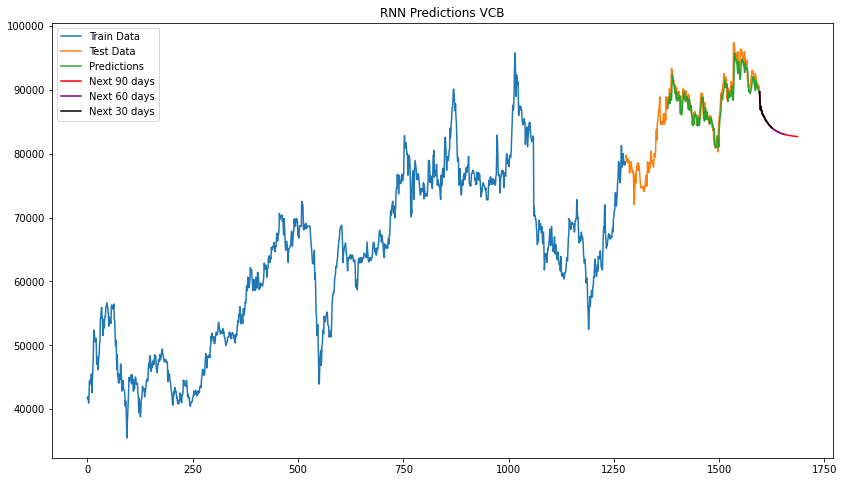
\includegraphics[width=\linewidth]{images/RNN/RNN_VCB_82.png}
    \captionof{figure}{RNN 8:2}
    \label{fig:image1}
\end{minipage}
\hfill
\begin{minipage}{0.21\textwidth}
    \centering
    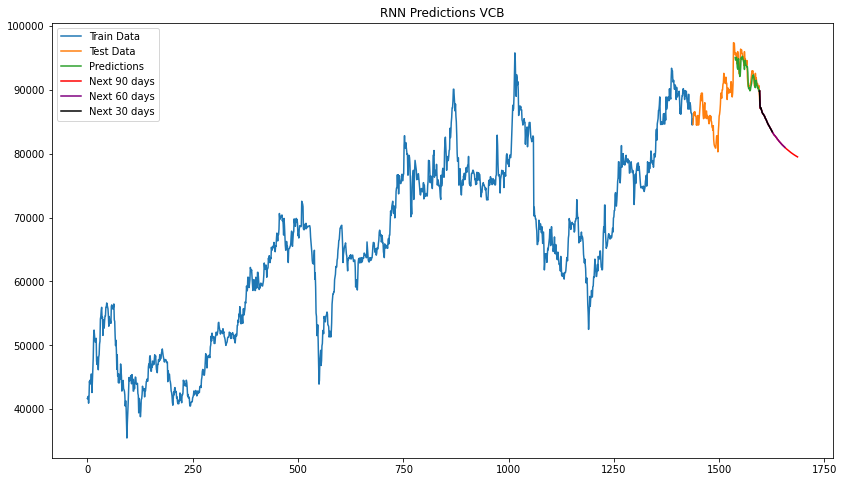
\includegraphics[width=\linewidth]{images/RNN/RNN_VCB_91.png}
    \captionof{figure}{RNN 9:1}
    \label{fig:image2}
\end{minipage}

\begin{minipage}{0.21\textwidth}
    \centering
    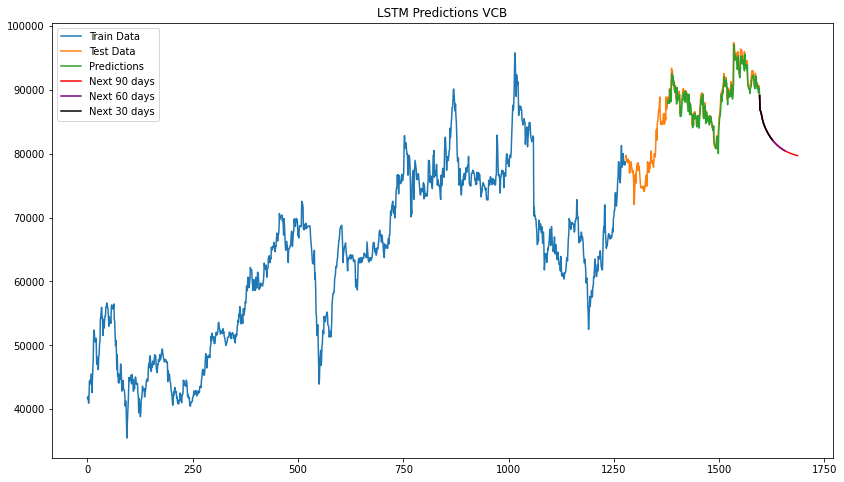
\includegraphics[width=\linewidth]{images/LSTM/LSTM_VCB_82.png}
    \captionof{figure}{LSTM 8:2 }
    \label{fig:image1}
\end{minipage}
\hfill
\begin{minipage}{0.21\textwidth}
    \centering
    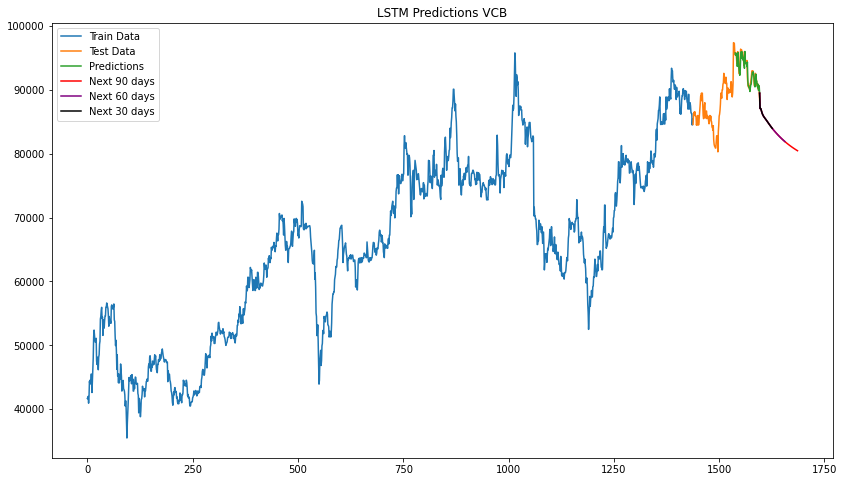
\includegraphics[width=\linewidth]{images/LSTM/LSTM_VCB_91.png}
    \captionof{figure}{LSTM 9:1}
    \label{fig:image2}
\end{minipage}

\begin{minipage}{0.21\textwidth}
    \centering
    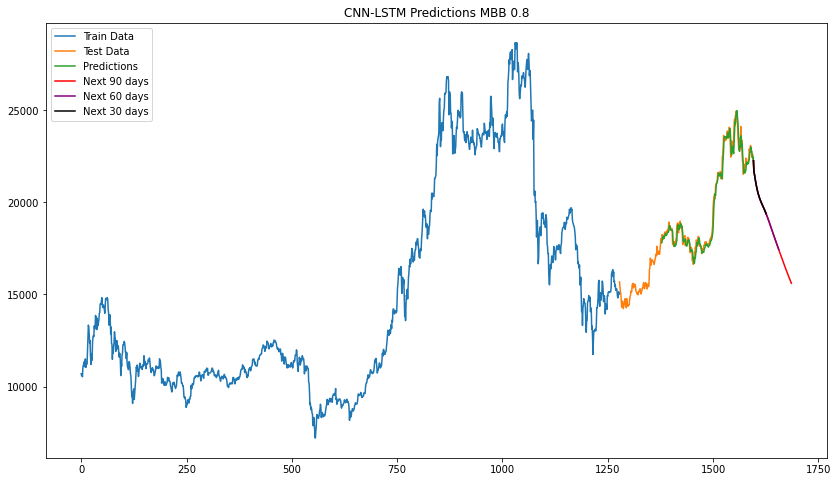
\includegraphics[width=\linewidth]{images/CNN-LSTM/CNNLSTM_VCB_82.png}
    \captionof{figure}{CNN-LSTM 8:2}
    \label{fig:image1}
\end{minipage}
\hfill
\begin{minipage}{0.21\textwidth}
    \centering
    \includegraphics[width=\linewidth]{images/CNN-LSTM/CNNLSTM_VCB_91.png}
    \captionof{figure}{CNN-LSTM 9:1}
    \label{fig:image2}
\end{minipage}

\begin{minipage}{0.21\textwidth}
    \centering
    \includegraphics[width=\linewidth]{images/MICN/MICN_VCB_82.png}
    \captionof{figure}{MICN 8:2}
    \label{fig:image1}
\end{minipage}
\hfill
\begin{minipage}{0.21\textwidth}
    \centering
    \includegraphics[width=\linewidth]{images/MICN/MICN_VCB_91.png}
    \captionof{figure}{MICN 9:1 }
    \label{fig:image2}
\end{minipage}





\subsubsection{ĐÁNH GIÁ TRÊN BỘ DỮ LIỆU MBB}

\begin{minipage}{0.21\textwidth}
    \centering
    \includegraphics[width=\linewidth]{images/LR/LR_MBB_82.png}
    \captionof{figure}{LR 8:2}
    \label{fig:image1}
\end{minipage}
\hfill
\begin{minipage}{0.21\textwidth}
    \centering
    \includegraphics[width=\linewidth]{images/LR/LR_MBB_91.png}
    \captionof{figure}{LR 9:1}
    \label{fig:image2}
\end{minipage}

\begin{minipage}{0.21\textwidth}
    \centering
    \includegraphics[width=\linewidth]{images/Holt Winter/HW_MBB_82.png}
    \captionof{figure}{Holt-Winter 8:2}
    \label{fig:image1}
\end{minipage}
\hfill
\begin{minipage}{0.21\textwidth}
    \centering
    \includegraphics[width=\linewidth]{images/Holt Winter/HW_MBB_91.png}
    \captionof{figure}{Holt-Winter 9:1}
    \label{fig:image2}
\end{minipage}

\begin{minipage}{0.21\textwidth}
    \centering
    \includegraphics[width=\linewidth]{images/ARIMA/ARIMA_MBB_82.png}
    \captionof{figure}{ARIMA 8:2}
    \label{fig:image1}
\end{minipage}
\hfill
\begin{minipage}{0.21\textwidth}
    \centering
    \includegraphics[width=\linewidth]{images/ARIMA/ARIMA_MBB_91.png}
    \captionof{figure}{ARIMA 9:1}
    \label{fig:image2}
\end{minipage}

\begin{minipage}{0.21\textwidth}
    \centering
    \includegraphics[width=\linewidth]{images/XGBoost/XGBoost_MBB_82.png}
    \captionof{figure}{XGBoost 8:2}
    \label{fig:image1}
\end{minipage}
\hfill
\begin{minipage}{0.21\textwidth}
    \centering
    \includegraphics[width=\linewidth]{images/XGBoost/XGBoost_MBB_91.png}
    \captionof{figure}{XGBoost 9:1 }
    \label{fig:image2}
\end{minipage}

\begin{minipage}{0.21\textwidth}
    \centering
    \includegraphics[width=\linewidth]{images/LR CalendarFourier, DeterministicProcess/LRCD_MBB_82.png}
    \captionof{figure}{Linear Regression CalendarFourier, DeterministicProcess 8:2}
    \label{fig:image1}
\end{minipage}
\hfill
\begin{minipage}{0.21\textwidth}
    \centering
    \includegraphics[width=\linewidth]{images/LR CalendarFourier, DeterministicProcess/LRCD_MBB_91.png}}
    \captionof{figure}{Linear Regression CalendarFourier, DeterministicProcess 9:1}
    \label{fig:image2}
\end{minipage}

\begin{minipage}{0.21\textwidth}
    \centering
    \includegraphics[width=\linewidth]{images/GRU/GRU_MBB_82.png}
    \captionof{figure}{GRU 8:2 }
    \label{fig:image1}
\end{minipage}
\hfill
\begin{minipage}{0.21\textwidth}
    \centering
    \includegraphics[width=\linewidth]{images/GRU/GRU_MBB_91.png}
    \captionof{figure}{GRU 9:1 }
    \label{fig:image2}
\end{minipage}

\begin{minipage}{0.21\textwidth}
    \centering
    \includegraphics[width=\linewidth]{images/RNN/RNN_MBB_82.png}
    \captionof{figure}{RNN 8:2}
    \label{fig:image1}
\end{minipage}
\hfill
\begin{minipage}{0.21\textwidth}
    \centering
    \includegraphics[width=\linewidth]{images/RNN/RNN_MBB_91.png}
    \captionof{figure}{RNN 9:1}
    \label{fig:image2}
\end{minipage}

\begin{minipage}{0.21\textwidth}
    \centering
    \includegraphics[width=\linewidth]{images/LSTM/LSTM_MBB_82.png}
    \captionof{figure}{LSTM 8:2}
    \label{fig:image1}
\end{minipage}
\hfill
\begin{minipage}{0.21\textwidth}
    \centering
    \includegraphics[width=\linewidth]{images/LSTM/LSTM_MBB_91.png}
    \captionof{figure}{LSTM 9:1}
    \label{fig:image2}
\end{minipage}

\begin{minipage}{0.21\textwidth}
    \centering
    \includegraphics[width=\linewidth]{images/CNN-LSTM/CNNLSTM_MBB_82.png}
    \captionof{figure}{CNN-LSTM 8:2}
    \label{fig:image1}
\end{minipage}
\hfill
\begin{minipage}{0.21\textwidth}
    \centering
    \includegraphics[width=\linewidth]{images/CNN-LSTM/CNNLSTM_MBB_91.png}
    \captionof{figure}{CNN-LSTM 9:1}
    \label{fig:image2}
\end{minipage}

\begin{minipage}{0.21\textwidth}
    \centering
    \includegraphics[width=\linewidth]{images/MICN/MICN_MBB_82.png}
    \captionof{figure}{MICN 8:2}
    \label{fig:image1}
\end{minipage}
\hfill
\begin{minipage}{0.21\textwidth}
    \centering
    \includegraphics[width=\linewidth]{images/MICN/MICN_MBB_91.png}
    \captionof{figure}{MICN 9:1}
    \label{fig:image2}
\end{minipage}

\subsection{SO SÁNH, ĐÁNH GIÁ}

\begin{table*}[t]
\centering
\caption{ĐÁNH GIÁ TRÊN CÁC BỘ DỮ LIỆU}
\begin{tabular}{lcccccccccc}
\toprule
\multirow{2}{*}{\textbf{Tỉ lệ}} & \multirow{2}{*}{\textbf{Mô hình}} & \multicolumn{3}{c}{\textbf{BIDV}} & \multicolumn{3}{c}{\textbf{VCB}} & \multicolumn{3}{c}{\textbf{MBB}} \\ 
\cmidrule(lr){3-5} \cmidrule(lr){6-8} \cmidrule(lr){9-11}
 &  & \textbf{RMSE} & \textbf{MAE} & \textbf{MAPE (\%)} & \textbf{RMSE} & \textbf{MAE} & \textbf{MAPE (\%)} & \textbf{RMSE} & \textbf{MAE} & \textbf{MAPE (\%)} \\ 
\midrule
\multirow{10}{*}{7:3} 
                    & Linear Regression & 5106.099 & 4029.223 & 10.7 & 13314.847 & 11406.7 & 15.909 & 7754.886 & 7467.216 & 44.473\\
                    & Holt-Winter & 12147.353 & 10425.494 & 24.37 & 19660.67 & 16922.62 & 19.86 & 3030.488 & 2326.928 & 12.583\\
                    & ARIMA & 11644.413 & 9900.365 & 23.084 & 18989.785 & 16338.678 & 19.18 & 2971.378 & 2288.123 & 12.492\\
                    & XGBoost & 1531.03 & 782.56 & 1.69 & \textbf{1223.78} & \textbf{793.18} & \textbf{0.96} & \textbf{285.05} & \textbf{217.39} & \textbf{1.2}\\
                    & Linear & & & \\
                    & CalendarFourier, & 4643.148 & 3800.978 & 10.1 & 13837.12 & 11888.17 & 16.518 & 7823.866 & 7539.177 & 44.75\\
                    & DeterministicProcess & & & \\
                    & RNN & 848.758 & 610.66 & 1.444 & 1238.266 & 903.622 & 1.1\\
                    & GRU &  \textbf{799.344} &  \textbf{565.852} &  \textbf{1.3439} & 1505.262 & 1187.511 & 1.42 & 322.462 & 230.585 & 1.284\\
                    & LSTM & 1140.567 & 943.25 & 2.215 & 1626.77 & 1346.2 & 1.636 & 364.172 & 262.703 & 1.48\\
                    & CNN-LSTM & 818.416 & 579.635 & 1.374 & 1456.85 & 1133.341 & 1.349 & 357.54 & 269.474 & 1.515\\
                    & MICN & 4768.2027 & 3880.841 & 8.99 & 7171.965 & 6384.823 & 7.61 & 1455.6243 & 1397.8943 & 8.16\\
                    \midrule
\multirow{10}{*}{8:2} 
                    & Linear Regression & 5959.578 & 4485.368 & 9.618 & 4906.916 & 4224.515 & 4.829 & 3895.731 & 4385.594 & 22.978\\
                    & Holt-Winter & 5442.702 & 4004.039 & 8.67 & 9729.256 & 8419.695 & 9.45 & 4675.115 & 3715.823 & 18.094\\
                    & ARIMA & 5465.229 & 3899.99 & 8.384 & 9568.17 & 8264.83 & 9.26 & 4690.713 & 3730.365 & 18.162\\
                    & XGBoost & 1835.20 & 1056.32 & 2.19 & 1481.31 & 894.92 & 0.99 & \textbf{304.36} & \textbf{196.86} & \textbf{0.98}\\
                    & Linear  \\
                    & CalendarFourier, & 5034.1 & 3829.7 & 8.3 & 5144.08 & 4441.966 & 5.133 & 4836.991 & 4364.947 & 25.582\\
                    & DeterministicProcess & & & \\
                    & RNN & 903.898 & 652.472 & 1.44 & 1525.8 & 1123.53 & 1.249 \\
                    & GRU & \textbf{778.219} & \textbf{550.714} & \textbf{1.233} & 1292.515 & 964.056 & 1.076 & 316.972 & 224.028 & 1.097\\
                    & LSTM & 863.893 & 631.665 & 1.41 & \textbf{1170.171} & \textbf{869.401} & \textbf{0.969} & 309.524 & 219.665 & 1.075\\
                    & CNN-LSTM & 819.226 & 581.721 & 1.301 & 342.531 & 251.857 & 1.235 & 333.924 & 245.384 & 1.201\\
                    & MICN & 5851.538 & 4515.326 & 9.73 & 13536.513 & 13263.265 & 15.24 & 700.2225 & 619.9381 & 3.57\\
                    \midrule
\multirow{10}{*}{9:1} 
                    & Linear Regression & 7397.376 & 6358.285 & 13.152 & 4402.437 & 3575.22 & 3.911 & 2318.005 & 2037.823 & 10.3597\\
                    & Holt-Winter & 9974.911 & 8400.13 & 17.107 & 6184.328 & 5317.27 & 5.84 & 3873.053 & 3092.189 & 13.75 \\
                    & ARIMA & 10578.949 & 8939.392 & 18.199 & 5997.686 & 4922.698 & 5.36 & 3928.862 & 3100.638 & 13.732\\
                    & XGBoost & 2631.97 & 1757.3 & 3.47  & 1571.18 & 988.49 & 1.06 & \textbf{360.88} & \textbf{260.76} & \textbf{1.21}\\
                    & Linear & & & \\
                    & CalendarFourier, & 5719.048 & 4611.46 & 9.4 & 4474.24 & 3779.58 &4.179 & 1851.396 & 1628.438 & 8.37\\
                    & DeterministicProcess & & & \\
                    & RNN & 1035.685 & 763.267 & 1.489 & 1076.603 & 801.1 & 0.856 & 466.864 & 370.408 & 1.604\\
                    & GRU & \textbf{946.578} & \textbf{644.264} & \textbf{1.262}  & 879.522 & 684.756 & 0.735 & 443.137 & 351.169 & 1.516\\
                    & LSTM & 991.127 & 723.549 & 1.418 & \textbf{848.022} & \textbf{649.84} & \textbf{0.696} & 424.367 & 329.62 & 1.421\\
                    & CNN-LSTM & 476.62 & 375.372 & 1.633 & 1153.785 & 879.134 & 0.943 & 542.099 & 441.47 & 1.907\\
                    & MICN  & 7823.79 & 6982.51 & 14.54 & 14089.16 & 13939.425 & 15.53 & 1057.8475 & 952.3056 & 4.84\\
                    \bottomrule
\end{tabular}
\end{table*}

\text{   
   
}
\section{KẾT LUẬN}
\subsection{KẾT LUẬN TỔNG THỂ}
Cổ phiếu mang đến những cơ hội đầu tư tuyệt vời nhưng cũng đi kèm với những rủi ro do tính chất khó lường của chúng. Tuy nhiên, những tiến bộ trong các phương pháp thống kê, thuật toán học máy và học sâu đã mở đường cho sự phát triển của các mô hình dự đoán có độ chính xác cao.\\
Kết quả nghiên cứu của nhóm cho thấy thuật toán XGBoost, GRU và LSTM là phù hợp nhất trong việc dự đoán giá cổ phiếu
trong tương lai của 3 ngân hàng BIDV, VCB, MBB. \\
Cụ thể, XGBoost dự báo tốt nhất cho ngân hàng MBB trong mọi tỉ lệ. Theo sau là thuật toán LSTM và GRU\\
Đối với dữ liệu ngân hàng VCB, các kết quả có sự phân bố đa dạng ở các mô hình và tỉ lệ phân chia tập dữ liệu. Trong đó mô hình XGBoost đạt hiệu suất tốt nhất trên tỉ lệ 7:3, theo sau là mô hình RNN. Mô hình LSTM tốt nhất trên cả 2 tỉ lệ 8:2 và 9:1.\\
Đối với dữ liệu ngân hàng BIDV, GRU lại cho kết quả tốt nhất ở cả ba tỉ lệ. Theo sau là CNN-LSTM ở 2 tỉ lệ 7:3 và 8:2.\\
Cuối cùng, thực hiện trực quan kết quả dự báo bằng biểu đồ, trong đó chứa thông tin dự báo trong 30-60-90 ngày tiếp theo trong tương lai.

\subsection{KHÓ KHĂN, THÁCH THỨC}
Mặc dù trong quá trình thực hiện đồ án nhóm đã cố gắng tìm hiểu đào sâu lý thuyết để triển khai các mô hình một cách tốt nhất có thể nhưng nhóm nghiên cứu vẫn nhận sự bản thân còn thiếu kinh nghiệm và kiến thức để triển khai các thuật toán đó một cách hoàn chỉnh nhất. 
\begin{itemize}
    \item Chưa thông thạo kiến thức về lập trình: Trong quá trình thực hiện đồ án, ngôn ngữ lập trình được sử dung là Python - một ngôn ngữ mà nhóm nghiên cứu lần đầu sử dung vì vậy việc vừa tìm hiểu ngôn ngữ mới vừa áp dụng nó để triền khai các thuật toán là môt thách thức không nhỏ đối với nhóm nghiên cứu.
    \item Nguồn dữ liệu có tính phù hợp khác nhau với mỗi thuật toán: Nhóm nghiên cứu nhận thấy với đa số các mô hình nhóm thực hiện dữ liệu của ngân hang MBB các tính phù hợp cao nhất, cho ra những kết quả đánh giá tốt nhất, còn với 2 ngân hàng còn lại vẫn có những mô hình chứ thể dự đoán ra kết quả tốt, vậy nên có thể phải xử lý những dữ liệu của các ngân hàng tốt hơn để thu được kết quả tốt cho các mô hình và dự liệu khác nhau.
    \item Việc sử dung một thuộc tính giá duy nhất để dự đoán giá cổ phiếu khi trên thực tế có rất nhiều yếu tố tác động dẫn đến việc dữ lieu dự đoán cho tương lai có phần chưa chính xác với thực tế cũng là một thách thức cần được xem xét cho nhóm nghiên cứu. 
\end{itemize}

\subsection{ĐỊNH HƯỚNG TRONG TƯƠNG LAI}
Bằng kinh nghiệm thực hiện đồ án môn Phân tích dữ liệu kinh doanh, chúng em sẽ tìm hiểu sâu hơn về cách các thuật toán hoạt động, kết hợp những điểm mạnh của các thuật toán để áp dụng với đúng bộ dữ liệu phù hợp.\\
Nhóm sẽ tập trung cải thiện hiệu suất của các mô hình qua việc tinh chỉnh các siêu tham số cũng như kiến trúc lớp của những mô hình như CNN-LSTM, MICN để nâng cao tính chính xác của mô hình.
Nhóm cũng sẽ thực nghiệm thêm với những mô hình mới và thêm nhiều bộ dữ liệu, nhất là với những dữ liệu biến động do các yếu tố bất ngờ (kinh doanh thua lỗ, nợ xấu) để tăng tính thực tế.\\
Với mục tiêu đảm bảo các mô hình có độ chính xác cao hơn và phù hợp với từng bộ dữ liệu.

\subsection{LỜI CẢM ƠN}
Với lòng biết ơn sâu sắc nhất, nhóm xin gửi lời cảm ơn chân thành và sâu sắc tới PGS. TS. Nguyễn Đình Thuân, GVTG Nguyễn Minh Nhựt đã tận tâm hướng dẫn, hỗ trợ qua từng buổi học trên lớp, giải đáp kịp thời các thắc mắc của nhóm, đưa ra những góp ý để nhóm có thể hoàn thành đồ án môn học và đạt được kết quả đề ra.

\printbibliography

\end{document}
